% !TEX TS-program = xelatex
% !BIB program = bibtex
% !TeX spellcheck = ru_RU

% About magic macros see also
% https://tex.stackexchange.com/questions/78101/

% По умолчанию используется шрифт 14 размера.
% Если Вы не влезаете в лимит страниц и нужен 12-й шрифт,
% то уберите опцию [14pt]
\documentclass[14pt, russian]{tex/matmex-diploma-custom}

\begin{document}
% !TeX spellcheck = ru_RU
% !TEX root = vkr.tex

%% Если что-то забыли, при компиляции будут ошибки Undefined control sequence \my@title@<что забыли>@ru
%% Если англоязычная титульная страница не нужна, то ее можно просто удалить.
\filltitle{ru}{
    %% Актуально только для курсовых/практик. ВКР защищаются не на кафедре а в ГЭК по направлению,
    %%   и к моменту защиты вы будете уже не в группе.
    chair              = {Кафедра информатики},
    group              = {23.М04-мм},
    %
    %% Макрос filltitle ненавидит пустые строки, поэтому обязателен хотя бы символ комментария на строке
    %% Актуально всем.
    title              = {Определение кода Голланда по результатам психометрических тестов личности на основе методов машинного обучения в условиях неполноты информации},
    %
    %% Здесь указывается тип работы. Возможные значения:
    %%   production - производственная практика;
    %%   coursework - отчёт по курсовой работе (ОБРАТИТЕ ВНИМАНИЕ, у техпрога и ПИ нет курсовых, только практики);
    %%   practice - отчёт по учебной практике;
    %%   prediploma - отчёт по преддипломной практике;
    %%   master - ВКР магистра;
    %%   bachelor - ВКР бакалавра.
    type               = {master},
    %
    %% Здесь указывается вид работы. От вида работы зависят критерии оценивания.
    %%   solution - «Решение». Обучающемуся поручили найти способ решения проблемы в области разработки программного обеспечения или теоретической информатики с учётом набора ограничений.
    %%   experiment - «Эксперимент». Обучающемуся поручили изучить возможности, достоинства и недостатки новой технологии, платформы, языка и т. д. на примере какой-то задачи.
    %%   production - «Производственное задание». Автору поручили реализовать потенциально полезное программное обеспечение.
    %%   comparison - «Сравнение». Обучающемуся поручили сравнить несколько существующих продуктов и/или подходов.
    %%   theoretical - «Теоретическое исследование». Автору поручили доказать какое-то утверждение, исследовать свойства алгоритма и т.п., при этом не требуя написания кода.
    kind               = {solution},
    %
    author             = {ГЛУШКОВ Егор Александрович},
    %
    %% Актуально только для ВКР. Указывается код и название направления подготовки. Типичные примеры:
    %%   02.03.03 \enquote{Математическое обеспечение и администрирование информационных систем}
    %%   02.04.03 \enquote{Математическое обеспечение и администрирование информационных систем}
    %%   09.03.04 \enquote{Программная инженерия}
    %%   09.04.04 \enquote{Программная инженерия}
    %% Те, что с 03 в середине --- бакалавриат, с 04 --- магистратура.
    specialty          = {02.04.03 \enquote{Математическое обеспечение и администрирование информационных систем}},
    %
    %% Актуально только для ВКР. Указывается шифр и название образовательной программы. Типичные примеры:
    %%   СВ.5162.2020 \enquote{Технологии программирования}
    %%   СВ.5080.2020 \enquote{Программная инженерия}
    %%   ВМ.5665.2022 \enquote{Математическое обеспечение и администрирование информационных систем}
    %%   ВМ.5666.2022 \enquote{Программная инженерия}
    %% Шифр и название программы можно посмотреть в учебном плане, по которому вы учитесь.
    %% СВ.* --- бакалавриат, ВМ.* --- магистратура. В конце --- год поступления (не обязательно ваш, если вы были в академе/вылетали).
    programme          = {ВМ.5665.2023 \enquote{Математическое обеспечение и администрирование информационных систем}},
    %
    %% Актуально всем.
    %% Должно умещаться в одну строчку, допускается использование сокращений, но без переусердствования,
    %% короткая строка с большим количеством сокращений выглядит странно
    %supervisorPosition = {проф. кафeдры системного программирования, д.ф.-м.н.,}, % Терехов А. Н.
    %supervisorPosition = {ст. преподаватель кафедры ИАС, к.~ф.-м.~н. (если есть),}, % Смирнов К. К.
    supervisorPosition = {доцент кафедры информатики, к.~т.~н.,},
    supervisor         = {Абрамов~М.~В.},
    %
    %% Актуально только для практик и курсовых. Если консультанта нет или он совпадает с научником, закомментировать или удалить вовсе.
    consultantPosition = {ст. преподаватель кафедры информатики,},
    consultant         = {Столярова~В.~Ф.},
    %
    %% Актуально только для ВКР.
    reviewerPosition   = {ст. научный сотрудник, СПб~ФИЦ~РАН, к.~т.~н.,},
    reviewer           = {Захаров~В.~В.},
}

% Английский титульник нужен только для ВКР, остальные виды работ могут его смело игнорировать.
\filltitle{en}{
    chair              = {Advisor's chair},
    group              = {ХХ.BХХ-mm},
    title              = {Determination of the Holland Code based оn the results of psychometric personality tests using machine learning methods in the presence of incomplete information},
    type               = {master},
    author             = {Egor Glushkov},
    %
    %% Possible choices:
    %%   02.03.03 \foreignquote{english}{Software and Administration of Information Systems}
    %%   02.04.03 \foreignquote{english}{Software and Administration of Information Systems}
    %%   09.03.04 \foreignquote{english}{Software Engineering}
    %%   09.04.04 \foreignquote{english}{Software Engineering}
    %% Те, что с 03 в середине --- бакалавриат, с 04 --- магистратура.
    specialty          = {02.04.03 \foreignquote{english}{Software and Administration of Information Systems}},
    %
    %% Possible choices:
    %%   СВ.5162.2020 \foreignquote{english}{Programming Technologies}
    %%   СВ.5080.2020 \foreignquote{english}{Software Engineering}
    %%   ВМ.5665.2022 \foreignquote{english}{Software and Administration of Information Systems}
    %%   ВМ.5666.2022 \foreignquote{english}{Software Engineering}
    programme          = {ВМ.5665.2023 \foreignquote{english}{Software and Administration of Information Systems}},
    %
    %% Note that common title translations are:
    %%   кандидат наук --- C.Sc. (NOT Ph.D.)
    %%   доктор ... наук --- Sc.D.
    %%   доцент --- docent (NOT assistant/associate prof.)
    %%   профессор --- prof.
    supervisorPosition = {C.Sc., docent, Department of CS,},
    supervisor         = {M.~V.~Abramov},
    %
    consultantPosition = {senior lecturer, Department of CS,},
    consultant         = {V.~F.~Stoliarova},
    %
    reviewerPosition   = {C.Sc., senior researcher, SPb FRC RAS,},
    reviewer           = {V.~V.~Zakharov},
}

\maketitle
\setcounter{tocdepth}{2}
\tableofcontents

\pagebreak
\newfontfamily\myfont{CMU Sans Serif}

% !TeX spellcheck = ru_RU
% !TEX root = vkr.tex


\section*{Введение}

Многие аспекты успешности человека обусловлены корректным определением карьерного пути, который соответствует его личностным предпочтениям~\cite{Presti}. От того, насколько успешно человек определил свою социально-профессиональную направленность, зависит удовлетворенность человека своей работой~\cite{Aydıntan, Cannas, Medgyesi}. Карьерному самоопределению уделяются значительные ресурсы, в том числе со стороны государства~\cite{FZ489}, чьи усилия направляются в том числе на профессиональное образование людей, которые по окончании обучения не работают по своей специальности вследствие отсутствия интереса к выбранной профессии. С определением своего будущего с профессиональной точки зрения сталкивается любой выпускник школы и вуза, безработный, работник, не удовлетворенный текущей работой или уже находящийся в процессе её смены, — для всех этих категорий людей встает вопрос об определении своих профориентационных предпочтений. Золотым стандартом является глубинное интервью с экспертом, который поможет выявить сильные и слабые стороны личности. Однако этот подход является ресурсозатратным, и для автоматизации процесса профориентации используются дистанционные способы карьерного консультирования~\cite{Pordelan, Westman}, в том числе профориентационные тесты, доступные для прохождения онлайн и не требующие большого количества времени для прохождения~\cite{vk_psychotests}.

Одним из инструментов для определения профессиональных интересов уже более полувека является модель Дж. Голланда RIASEC~\cite{Holland1959}, которая предполагает, что профессиональные предпочтения являются отражением характера человека, его базовых черт. Так, вводятся шесть типов социально-профессиональной направленности личности (кодов Голланда): реалистический (Realistic, R), исследовательский (Investigative, I), артистический (Artistic, A), социальный (Social, S), предприимчивый (Enterprising, E) или традиционный (Conventional, C). Коды могут определяться при помощи тестирования, в котором в результате попарного сравнения профессий численно оцениваются указанные шесть типов направленности личности~\cite{Rezapkina}. Для сравнения профессиональных профилей личности (кодов Голланда) между собой используется C-индекс как мера сходства (конгруэнтности). Существует множество вариаций данного теста~\cite{Chu}, результаты которых коррелированы, однако не определяют друг друга однозначно. Кроме того, такие тесты часто не учитывают быстро изменяющуюся конъюнктуру рынка профессий, а также культурные и социо-экономические различия респондентов~\cite{Chu, Hoff, Nye}. Возникает актуальная задача определения кода Голланда по альтернативным данным.

В настоящее время существуют исследования, показывающие взаимосвязь кода Голланда индивида с его социально-демографическими признаками~\cite{Bogacheva}, цифровым следом в социальных сетях (его сообщения, посты, фото; в исследованиях могли быть использованы иные психометрические тесты)~\cite{Chekalev, Ivaschenko, Stoliarova, Oliseenko, Stankevich, Titov, Basaran}. Однако основное внимание исследователей направлено на изучение взаимосвязи факторов модели Голланда с факторами других психометрических тестов~\cite{Mason, Hurtado, Batista, Usslepp, Schuerger, Yamashita, Martins}. Для анализа взаимосвязей различных опросных инструментов исследователи используют методы регрессионного анализа и статистические тесты~\cite{Hurtado, Ivaschenko, Stoliarova}, моделирование структурными уравнениями (\emph{SEM})~\cite{Martins, Chu} и модели машинного обучения~\cite{Usslepp, Silva, Song, Bogacheva, Oliseenko, Stankevich, Titov, Basaran}.

Несмотря на наличие работ, в которых предсказывается результат одного психометрического теста на основе другого теста или на основе некоторых признаков личности (например, комментариев, постов и фото пользователей социальной сети), до сих пор нет инструментов, позволяющих по результатам одного или комбинации сразу нескольких популярных психометрических тестов (\enquote{Большая пятёрка}, Кеттелла, Айзенка, Леонгарда, Шварца) предсказывать код Голланда. Востребован инструмент, в котором результаты тестов могли бы быть предоставлены частично, который бы в меньшей степени зависел от изменяющейся конъюнктуры рынка профессий, от культурных и экономических различий респондентов, то есть позволял определять профессиональный профиль личности в условиях подобной неполноты информации. В результате, пользователь мог бы получить информацию о своих профориентационных предпочтениях без прохождения теста Голланда. Кроме того, даже при прохождении последнего подобный инструмент может использоваться для уточнения результатов теста Голланда и установления его непротиворечивости в соответствии с результатами других исследований.

Данная работа призвана закрыть этот пробел: с помощью современных методов машинного обучения на основе собранных данных по результатам прохождения одного или нескольких указанных психометрических тестов личности устанавливаются взаимосвязи между результатами тестов и предсказывается код Голланда, соответствующий профессиональным предпочтениям личности. Предсказание кода Голланда может быть решено такими методами машинного обучения, как многоцелевая регрессия, классификация или ранжирование~\cite{Bishop}; для улучшения качества прогноза базовые модели могут объединяться в ансамбли~\cite{ZhangC, Bischl}. Возможность предсказания по одному или нескольким тестам влечет необходимость восстановления результатов тестов, которые не были пройдены.

Новизна результатов исследования состоит в создании нового программного комплекса, обеспечивающего автоматизацию процесса профориентации на основе предсказания кода Голланда. Теоретическая значимость заключается в использовании уникальной комбинации различных психометрических тестов при разработке новых моделей машинного обучения для определения взаимосвязи тестов и кода Голланда. Практическая значимость~--- разработка прототипа программного модуля автоматизации оценки профессиональной направленности по психологическому профилю личности.

% !TeX spellcheck = ru_RU
% !TEX root = vkr.tex

\section{Постановка задачи}
\label{sec:task}

Целью работы является автоматизация процесса профориентации посредством разработки инструмента для предсказания кода Голланда по неполным результатам психометрических тестов с использованием методов машинного обучения.

\bigbreak
Для выполнения цели были поставлены следующие задачи:
\begin{enumerate}
    \item Разработать математическое обеспечение для модуля восстановления пропусков психометрических тестов.
    \item Реализовать различные подходы к определению кода Голланда: многоцелевая регрессия, классификация, ранжирование.
    \item Разработать модуль формирования взвешенного ансамбля моделей для объединения прогнозов базовых алгоритмов.
    \item Провести сравнительный анализ подходов и методов определения кода Голланда на основе C-индекса.
    \item Создать прототип инструмента для определения профориентационных предпочтений личности.
\end{enumerate}

% !TeX spellcheck = ru_RU
% !TEX root = vkr.tex

\section{Обзор}
\label{sec:relatedworks}

В данном разделе представлен обзор модели Голланда и дано краткое описание психометрических тестов личности. Проведен обзор предметной области: рассмотрены и проанализированы статьи, предлагающие различные подходы к решению задачи предсказания значений факторов психометрических тестов и нахождения взаимосвязей между факторами.

\subsection{Модель Голланда и психометрические тесты личности}
\subsubsection{Модель Голланда RIASEC}

Одним из основных инструментов оценки профессиональных интересов служит модель Голланда, также известная как модель \textit{RIASEC}. Данная методика была разработана Джоном Льюисом Голландом в конце 1950-х годов~\cite{Holland1959}, после чего им неоднократно дорабатывалась и развивалась. В своей статье \enquote{Теория профессионального выбора} исследователь сопоставляет различным типам личности профессиональные роды деятельности. Согласно Голланду, личности выбирают и преуспевают в той профессиональной среде, которая подходит их характеру, является отражением их базовых черт, при этом профессиональная карьерная среда классифицируется по тем типам личностей, которые в этой среде успешны. Таким образом, для определения профессиональных предпочтений достаточно определить социально-профессиональный тип личности.

В своих более поздних работах ученый выделяет следующие шесть типов личностей:
\begin{itemize}[noitemsep, topsep=0pt, parsep=0pt, partopsep=0pt]
  \item реалистический (\textit{Realistic}, R);
  \item исследовательский (\textit{Investigative}, I);
  \item артистический (\textit{Artistic}, A);
  \item социальный (\textit{Social}, S);
  \item предприимчивый (\textit{Enterprising}, E);
  \item традиционный (\textit{Conventional}, C).
\end{itemize}

При этом определяется не единственный тип личности: оценивается принадлежность человека к каждому из типов, которые затем выстраиваются в порядке убывания их выраженности. Результат записывается в виде кода по первым буквам типов, что и дало название модели. Модель Голланда также можно представить как правильный шестиугольник с кодами в вершинах (рисунок~\ref{fig:hexagon_RIASEC}).

\begin{figure}
    \centering
    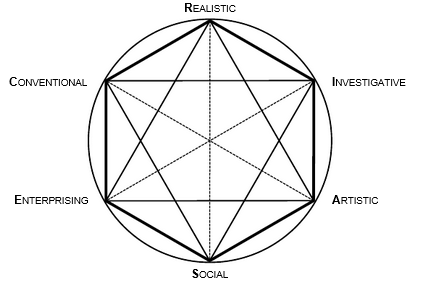
\includegraphics[width=0.65\linewidth]{figures/hexagon_RIASEC.png}
    \caption{Правильный шестиугольник, в вершинах которого расположены типы личности (коды) согласно Голланду\protect\footnotemark}
    \label{fig:hexagon_RIASEC}
\end{figure}

\footnotetext{Источник: Hexagonal arrangement of the RIASEC dimensions. URL: \url{https://www.researchgate.net/figure/Hexagonal-arrangement-of-the-RIASEC-dimensions_fig1_356677137}}

Существуют различные методики определения кода Голланда, и в российской адаптации методики Г.~В.~Резапкиной~\cite{Rezapkina} предлагается опросный инструмент с 42 парами профессий: из каждой пары опрашиваемый должен выбрать одну профессию, которая его более привлекает. Каждой из выбранных профессий сопоставляется один из шести типов, соответствие профессий и типов было произведено Голландом в своих работах и дополнено другими исследователями. Для каждого из типов подсчитывается количество упоминаний, и шесть типов выстраиваются в порядке убывания подсчитанных баллов. Например, опрашиваемый 11 раз в парах выбрал профессии, соответствующие исследовательскому типу (I), 10~--- традиционному (C), 9, 7, 5 и 0 предприимчивому (E), реалистическому (R), социальному (S) и артистическому (A) типам соответственно. Итоговым кодом для опрашиваемого будет \enquote{ICERSA}, который можно ограничить тремя первыми буквами (\enquote{верхняя триада}, \enquote{ICE}).

\label{subsec:cindex}
Для сравнения кода типа личности и кода его профессиональной среды Голланд вводит понятие конгруэнтности (согласованности). Среди мер согласованности можно выделить C‑индекс для трёхбуквенных кодов (\enquote{верхних триад}):
  \[
    C = 3\, (X_1, Y_1) + 2\, (X_2, Y_2) + 1\, (X_3, Y_3),
  \]
  где $\{X_i\}$ и $\{Y_i\}$ — первые три позиции кодов Голланда, их позиции в замкнутой цепочке (шестиугольнике) \textit{R-I-A-S-E-C}:
  \[
    (X_i, Y_i) =
    \begin{cases}
      3, & \text{если $X_i = Y_i$,}\\
      2, & \text{если $X_i$ и $Y_i$ -- соседние позиции,}\\
      1, & \text{если $X_i$ и $Y_i$ -- позиции через один код,}\\
      0, & \text{если $X_i$ и $Y_i$ -- противоположны.}
    \end{cases}
  \]
Б\'oльшие значения меры согласованности говорят о большем сходстве двух профессиональных профилей (кодов Голланда). 


\subsubsection{Психометрические тесты личности}
\label{sec:psytests}

Помимо модели Голланда есть и другие способы определения проф\-ори\-ента\-цион\-ных предпочтений. Одним из таких способов являются пси\-хо\-мет\-ри\-чес\-кие опросные инструменты. Их основная цель~--- отразить некоторые черты личности человека в удобном числовом формате. Они помогают выявить ключевые черты характера, тем\-пе\-ра\-мент, цен\-ности и по\-ве\-ден\-ческие особенности. 

Среди психометрических тестов личности можно выделить следующие (в скобках указано количество факторов):
    \begin{enumerate}[noitemsep, topsep=0pt, parsep=0pt, partopsep=0pt]
        \item Опросник Леонгарда-Шмишека (10).
        \item Личностный опросник Айзенка (4).
        \item 16-факторный опросник Кеттелла (16).
        \item Пятифакторный опросник личности (\enquote{Большая пятёрка}; 5).
        \item Ценностный опросник Шварца (20).
    \end{enumerate}

Опросник Леонгарда-Шмишека разработан Г.~Шмишеком на основе теории акцентуаций личности К.~Леонгарда~\cite{Schmieschek} (адаптация на русский язык~--- ~\cite{Kortneva}) и представляет собой опросник из 88 вопросов с ответами \enquote{да/нет}. Вопросы сгруппированы по 10 шкалам, по каждой из которых подсчитывается балл, отражающий выраженность соответствующей акцентуации. Методика позволяет составить индивидуальный психологический портрет, выявить усиленные черты характера, влияющие на поведение, эмоциональные реакции и адаптацию. Применяется в образовательных программах, при подборе персонала и профориентации.

Личностный опросник Айзенка (EPQ-R) разработан Г.~Айзенком и коллегами в 1985~г.~\cite{Eysenck} (русская адаптация Суходольского~\cite{Sukhodolsky}) и направлен на измерение базовых личностных параметров: экстраверсии, нейротизма, психотизма и оценки искренности ответов. Опросник включает 100 вопросов с ответами \enquote{да/нет}, по результатам которых формируются соответствующие шкалы, позволяющие оценить стиль взаимодействия человека с окружающим миром, его стрес\-со\-ус\-той\-чивость и темперамент. Методика широко применяется в клинической психологии, образовательных программах, профориентации и научных исследованиях.

16-факторный опросник Кеттелла (16PF)~\cite{Cattell} (адаптация~\cite{Shmelev}) предназначен для всесторонней диагностики личности через измерение 16 основных черт характера методом факторного анализа. Тест состоит из 187 вопросов с ответами \enquote{утвердительно}, \enquote{отрицательно} и \enquote{нейтрально}, что позволяет получить детальный личностный профиль. По итогам подсчитываются баллы по каждой из 16 шкал (от 0 до 26) и дополнительным шкалам, отражающим вторичные личностные особенности. Инструмент широко применяется при кадровом отборе, психологическом консультировании и научных исследованиях для глубокого понимания индивидуальных различий. Именно 16PF послужил основой для появления пятифакторных тестов (\enquote{Большая пятёрка}).

Пятифакторный опросник личности (\enquote{Большая пятёрка}, 5PFQ)~\cite{Tsuji} (русская адаптация Хромова~\cite{Khromov}) основан на модели факторного анализа \textit{NEO-PI-R}~\cite{Costa} и представляет собой диспозиционную методику для оценки пяти базовых черт личности: экстраверсия, привязанность, самоконтроль, эмоциональная устойчивость, экспрессивность. Тест включает 75 утверждений, которые оцениваются от –2 до 2, что позволяет получить итоговые шкалы, отражающие степень выраженности каждой черты, а также множество вторичных факторов. Инструмент широко применяется в профориентации, подборе персонала и научных исследованиях.

Ценностный опросник Шварца (SVS)~\cite{Schwartz} (русская адаптация Карандашева~\cite{Karandashev}) предназначен для количественной оценки 10 универсальных ценностей, выявленных методом исследования жизненных приоритетов. Методика использует парное сравнение ценностей и фиксирует две оценки: нормативный идеал (какие ценности человек считает важными в идеале) и индивидуальный приоритет (что важно для него лично). Опросник активно применяется в социологических и психологических исследованиях для анализа культурных различий и индивидуальных мотивационных профилей.


\subsection{Методы машинного обучения в вычислительной психологии личности}

Применению методов машинного обучения в вычислительной психологии личности (\emph{personality computing}) в целом и нахождению взаимосвязей результатов различных психометрических тестов между собой в частности посвящено множество научных работ. Для решения задачи установления взаимосвязи между факторами психологических тестов, а также внешними признаками используются следующие методы:

\begin{itemize}[noitemsep, topsep=0pt, parsep=0pt, partopsep=0pt]
  \item Статистические: регрессионный, корреляционный, факторный анализ; структурное моделирование (\emph{SEM}).
  \item Динамические: модели, описывающие изменения во времени (дифференциальные уравнения).
  \item Сетевые: анализ взаимосвязей между переменными как узлов в сети.
  \item Машинное обучение: классификация, кластеризация, регрессия, ранжирование.
\end{itemize}

Так, всё чаще встречается применение методов машинного обучения в вычислительной психологии. Задачи могут быть различны.
\begin{itemize}
    \item Предсказание кода Голланда на основе социально-демо\-графических признаков~\cite{Bogacheva}. Авторы предлагают различные подходы для решения этой задачи: с тех пор как код Голланда может быть представлен и как последовательно идущие три или шесть кодов, и как целочисленные значения кодов, то и задача может быть поставлена следующим образом: регрессия с множественными выходами (\textit{многоцелевая}; \emph{multi\-output regression}), классификация с несколькими метками (\emph{multi\-label classification}), классификация с множественными выходами (\emph{multi\-output classification}). Авторы отмечают: в случае последовательного предсказания для многоцелевой регрессии порядок предсказания выходов важен. В качестве меры сходства авторы используют меру конгруэнтности~--- C-индекс. Наилучшие результаты показал градиентный бустинг: $\text{C‑index} = 10.95$ при решении задачи регрессии и $\text{C‑index} = 11.08$ при решении задачи классификации.
    
    \item Оценка профессионального выбора~\cite{Song}. Пользователю по результатам прохождения теста Голланда предъявлялся список профессий, которым прежде уже был сопоставлен свой код Голланда; требовалось найти наиболее подходящие профессии. Наилучших результатов удалось достичь с помощью комбинации традиционных методов и ансамбля методов машинного обучения. В качестве традиционных методов использовалось сравнение значений мер конгруэнтности (простое совпадение главного фактора кода Голланда, оценка профилей~--- числовых значений кода Голланда~--- с помощью таких метрик, как коэффициент корреляции Пирсона и Евклидово расстояние). В ансамбль методов машинного обучения вошли следующие модели: многослойный перцептрон (нейронная сеть), метод k-ближайших соседей, регуляризованная регрессия, случайный лес.
    
    \item В статье~\cite{Usslepp} применяется логистическая регрессия для предсказания (классификации), какой путь выберут учащиеся: академический или профессиональный; предикторами служили значения факторов тестов Голланда и \enquote{Большой пятерки}.
    
    \item Расширение списка профессий, поставленных в соответствие кодам Голланда, путем создания платформы для автоматизации профилирования вакансий~\cite{Silva}. Предсказание кодов Голланда решается как задача ранжирования с метрикой NDCG (\textit{Normalized Discounted Cumulative Gain}).
    
    \item Предсказание значений шкал теста \enquote{Большой пятерки} пользователей социальных сетей по следующим признакам: их посты, комментарии, репосты и численные характеристики аккаунта пользователя. Решалась задача бинарной классификации (шкалы теста были представлены бинарными путем сравнения с пороговым значением) с использованием моделей случайного леса и метода опорных векторов~\cite{Stankevich}. Подобная задача в работе~\cite{Basaran} решалась с помощью многослойного перцептрона. По схожим признакам (в т.~ч. по указанной в профиле пользователя информации) для оценки темперамента (тест Айзенка EPQ) в статье~\cite{Oliseenko} использовались модели CatBoost и случайный лес. В работе~\cite{Titov} предсказание результатов тестов \enquote{Большой пятерки}, Шварца и других по извлекаемым из профилей в социальной сети численным признакам (число друзей, постов, подписок, длина поля с личным описанием, длина постов и др.) осуществляется с помощью модели XGBoost (\emph{eXtreme Gradient Boosting}).
\end{itemize}

\subsection{Выводы}

Для предсказания кода Голланда могут быть использованы различные идеи, рассмотренные в данном обзоре. Например, задачу можно сформулировать как регрессию/классификацию с множественными выходами (\emph{multioutput}), классификацию с несколькими метками (\emph{multilabel}). Для многоцелевой регрессии могут быть использованы различные метрики: не только усредненные MSE или RMSE, часто применяемые в таких задачах, но и специальные меры конгруэнтности (\textit{сходства}, C-индекс), косинусное расстояние, коэффициент корреляции. Приведены различные методы машинного обучения, в том числе и те, с помощью которых были достигнуты наилучшие результаты: в первую очередь, это градиентный бустинг (CatBoost, XGBoost) и случайный лес. В соответствии с результатами работы~\cite{Bogacheva} приемлемым может считаться следующий результат предсказания значений кода Голланда: $\text{C‑index} \geq 11$.

Несмотря на разнообразие работ, наличие среди них тех, где по результатам одних психометрических тестов предсказываются другие, до сих пор нет инструментов, позволяющих по результатам сразу нескольких популярных психометрических тестов~--- \enquote{Большой пятерки}, Кеттелла, Айзенка, Леонгарда, Шварца~--- предсказать код Голланда. Таким образом, пользователь мог бы получить информацию о своих профориентационных предпочтениях без прохождения теста Голланда. Кроме того, даже при прохождении последнего подобный инструмент мог бы уточнять результаты теста Голланда, проверять его непротиворечивость в соответствии с результатами других тестов.

% !TeX spellcheck = ru_RU
% !TEX root = vkr.tex

\section{Модели и методы определения кода Голланда по данным психометрических тестов}

В данном разделе описываются различные подходы к предсказанию кода Голланда на полных данных (без пропусков) и на данных с пропусками, требующими восстановления. В конце раздела приводится итоговая структура решения задачи по предсказанию кода Голланда.

\subsection{Определение кода Голланда на полных данных: регрессия, классификация, ранжирование}

Данные психометрических тестов представляют собой набор признаков, принимающих целочисленные значения. Пример данных психометрических тестов приведен в таблице~\ref{tab:input_test_data}. Определение кода Голланда представляет собой предсказание шести чисел, отражающих степень выраженности типов личности (кодов Голланда). В качестве альтернативы набору из шести чисел предсказанием кода может служить ответ как в виде однобуквенного значения, так и набора из трех букв, \enquote{верхней триады}~--- тройки наиболее выраженных кодов. В случае, если в таком наборе задан порядок, то речь может идти о предсказании рангов кодов (от менее выраженного к наиболее выраженному).

\begingroup
  \fontsize{7pt}{8pt}\selectfont
  \begin{table}[ht]
    \centering
    \caption{Пример данных психометрических тестов}
    \label{tab:input_test_data}
    \begin{tabular*}{\textwidth}{
      @{\extracolsep{\fill}} 
      >{\centering\arraybackslash}p{0.8cm}       |  % id
      *{3}{>{\centering\arraybackslash}p{1.1cm}}    % BF
      >{\centering\arraybackslash}p{0.3cm}          % ...
      *{2}{>{\centering\arraybackslash}p{1.2cm}} |  % LN
      *{6}{>{\centering\arraybackslash}p{0.9cm}}    % HL
    }
        \toprule
        \multirow{2}{*}{\textbf{id}}
        & \multicolumn{3}{c}{\textbf{Бол. пятёрка}}
        & \multirow{2}{*}{\textbf{\dots}}
        & \multicolumn{2}{c|}{\textbf{Леонгард}}
        & \multicolumn{6}{c}{\textbf{Голланд}} \\
        \cmidrule(lr){2-4} \cmidrule(lr){6-7} \cmidrule(lr){8-13}
        & BF1 & BF2 & BF3 
        & 
        & LN9 & LN10 
        & HL1 & HL2 & HL3 & HL4 & HL5 & HL6 \\
        \midrule
        1 & 39 & 66 & 33 & \dots &  3 & 12  &  8 &  8 &  6 &  8 &  1 & 11 \\
        2 & 45 & 46 & 73 & \dots & 12 &  6  &  3 &  7 &  7 &  8 & 10 &  7 \\
        3 & 34 & 41 & 56 & \dots & 18 & 12  & 10 & 10 &  3 & 11 &  7 &  1 \\
        4 & 49 & 47 & 50 & \dots & 15 & 24  &  6 &  4 &  8 &  6 &  7 & 11 \\
        5 & 48 & 42 & 53 & \dots & 12 &  6  &  6 &  7 &  8 &  7 & 10 &  4 \\
        \bottomrule
    \end{tabular*}
  \end{table}
\endgroup

Таким образом, задача определения кода Голланда по результатам психометрических тестов личности может быть сведена к следующим задачам:
\begin{enumerate}[label={\arabic*)}]
    \item регрессия со множественными выходами (набор чисел);
    \item классификация (набор кодов);
    \item ранжирование (упорядоченный набор кодов);
    \item ансамблевые модели (комбинация базовых моделей).
\end{enumerate}


\subsubsection{Регрессия}
\label{subsec:regr}

Предсказание сразу нескольких целевых числовых переменных представляет собой регрессию со множественными выходами (многоцелевая регрессия, \emph{multitarget}). Существует три основных подхода к решению данной задачи~\cite{Spyromitros, Bishop}:
\begin{itemize}
    \item Применение моделей, по умолчанию поддерживающих множественные выходы (линейная регрессия, метод k-ближайших соседей, нейронные сети).
    \item Независимые предсказания каждого из выходов (\emph{multioutput}).
    \item Предсказания выходов по цепочке: последний предсказанный выход становится частью признакового пространства для предсказания следующего выхода (\emph{regressor chain}, см. рисунок \ref{fig:multioutput_regr}).
\end{itemize}

\begin{figure}[ht]
    \centering
    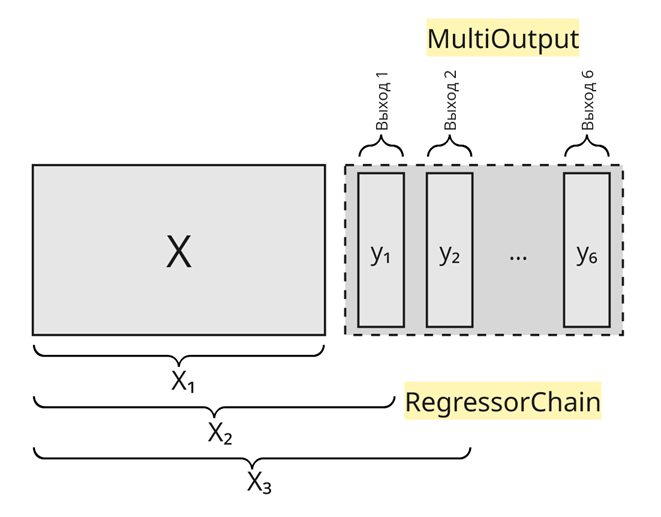
\includegraphics[width=0.75\linewidth]{figures/multioutput.png}
    \caption{Многоцелевая регрессия}
    \label{fig:multioutput_regr}
\end{figure}

Оцениваются результаты решения задачи регрессии со множественными выходами с помощью следующих усредненных по ответам метрик на тестовой выборке:
\begin{itemize}
    \item усредненная среднеквадратичная ошибка (RMSE);
    \item усредненный C-индекс (мера сходства, см. \ref{subsec:cindex}).
\end{itemize}

Лучшее качество обеспечивается при минимальных значениях RMSE и при максимальных значениях C-индекса (как мера согласованности). Чем больше С-индекс, тем большее сходство имеют два сравниваемых между собой профиля. Использование С-индекса позволяет сравнивать результаты не только с другими регрессионными задачами, но и, например, с задачами классификации. Стоит отметить, что в процессе обучения некоторые модели также позволяют оценить важность признаков: ансамблевые модели на основе решающих деревьев (случайный лес, градиентные бустинги) и линейные регрессоры.

Для нахождения взаимосвязей между факторами модели Голланда и другими психометрическими тестами в качестве базовых были использованы следующие регрессионные модели:
\begin{itemize}
    \item модели на основе линейной регрессии (простая линейная, пошаговая, L1-~и \mbox{L2-ре}\-гуля\-ризо\-ванные модели регрессии);
    \item модели на основе ансамблей деревьев с бутстрэппингом (случайный лес Random Forest, ExtraTrees);
    \item модели градиентного бустинга (XGBoost, LightGBM, CatBoost);
    \item непараметрические модели (kNN, SVR);
    \item нейросетевые модели (MLP, \emph{foundation-модель} TabPFN);
    \item базовая константная модель для сравнительного анализа.
\end{itemize}

При отсутствии пропусков (то есть при работе с \enquote{полными} данными) может быть целесообразным уменьшение размерности с помощью метода главных компонент (англ. \emph{Principal Component Analysis}, PCA)~\cite{Bishop}. Некоторые факторы различных тестов могут оценивать одни и те же аспекты личности, среди связей могут наблюдаться корреляции. Уменьшение размерности позволяет агрегировать схожие факторы тестов.


\subsubsection{Классификация}
\label{subsec:classif}

Предсказание одной или нескольких категориальных переменных (кодов, классов, меток) представляет собой задачу классификации. Предсказание кода Голланда как решение задачи классификации может быть сведено к следующим подходам~\cite{ZhangMin} (таблица~\ref{tab:class_types}):
\begin{itemize}
    \item Многоклассовая (\emph{multiclass}) классификация.\\
    Обучается один классификатор на шесть классов. В качестве ответа в порядке убывания вероятностей выбираются три наиболее вероятных кода.
    \item Многометочная (\emph{multilabel}) классификация.\\
    Обучаются шесть бинарных классификаторов, позволяющих дать ответ на вопрос, входит ли соответствующий код в \enquote{верхнюю триаду}. Выбираются три кода с наивысшими предсказанными вероятностями.
    \item Классификация на полное множество комбинаций (\emph{label powerset}).\\
    Всего существует 20 различных трехбуквенных комбинаций кода Голланда, в которых не учитывается порядок кодов. На выходе~--- тройка кодов. По причине отсутствия возможности учесть порядок кодов, для данного подхода невозможно использовать С-индекс, оценка которого основывается именно на порядке кодов.
\end{itemize}

\begingroup
\fontsize{7pt}{8pt}\selectfont
    \begin{table}[ht]
      \centering
      \caption{Подходы к классификации}
      \label{tab:class_types}
      \begin{tabular*}{0.95\textwidth}{@{\,}
        >{\centering\arraybackslash}m{3.8cm} |
        >{\centering\arraybackslash}m{4.2cm} |
        >{\centering\arraybackslash}m{4.5cm} |
        >{\centering\arraybackslash}m{2.5cm}}
        \toprule
        \textbf{Класси\-фикация}
          & \textbf{Модель}
          & \textbf{Значение}
          & \textbf{Пример} \\
        \midrule
        Много\-классовая (multiclass)
          & 1 классификатор на 6 классов
          & 3 однобуквенных кода
          & \texttt{R, S, E} \\
        \addlinespace[0.25em] \hline \addlinespace[0.25em]
        Много\-меточная (multilabel)
          & 6 бинарных классификаторов
          & Булевый вектор из 6 элементов с 3 значениями \texttt{True}
          & \texttt{[T, F, F, T, T, F]} \\
        \addlinespace[0.5em] \hline \addlinespace[0.25em]
        Множество комбинаций (label powerset)
          & 1 классификатор на 20 классов
          & трехбуквенный код, порядок кодов не важен
          & \texttt{RSE} \\
        \bottomrule
      \end{tabular*}
    \end{table}
\endgroup

По аналогии с решением задачи регрессии был применён метод главных компонент. Для оценки решения задачи классификации учитывалась метрика точности Top-K (\textit{Top-K accuracy}), которая показывает, в скольких случаях среди трех наиболее вероятных предсказанных моделью классов есть хотя бы \emph{K} правильно предсказанных меток. Например, $\text{Top-2}_{acc} = 0.7$ означает, что модель для 70\% предсказанных троек кодов угадала как минимум два истинных кода. Для сравнения с результатами других подходов также использовался \mbox{С-индекс}.

Для задачи классификации были взяты те же модели, что и для регрессии, за исключением нейросетевых моделей, а также с добавлением регуляризованных логистических регрессий (вместо линейных регрессий) и наивного байесовского классификатора.


\subsubsection{Ранжирование}
\label{subsec:ltr}

Представим задачу определения кода Голланда как задачу списочного ранжирования (\emph{listwise learn-to-rank})~\cite{Burges}. В отличие от поточечного ранжирования, где каждый элемент оценивается по шкале релевантности (что фактически сводится к задаче регрессии), или от попарного ранжирования, в котором моделируется относительный порядок пар элементов (бинарная классификация), списочное ранжирование рассматривает весь список результатов как единый упорядоченный объект.

Списочный подход требует задания двух ключевых компонентов: определения скоринговой функции и выбора функции потерь, оптимизирующей качество выдачи списка. В качестве скоринговой функции обычно используется многослойный перцептрон или более сложные архитектуры: глубокая перекрёстная сеть (\emph{Deep {\&} Cross Network}) либо трансформер с механизмом \emph{self‑attention}.

Типичными функциями потерь для списочного ранжирования являются NDCG (нормализованный дисконтированный совокупный прирост) и её дифференцируемые аппроксимации (ApproxNDCG, LambdaRank), а также специальные дифференцируемые функции, например ListNet, которая минимизирует кросс‑энтропию распределений релевантности и оптимизирует вероятность корректного попадания в топ‑k (в контексте решения задачи это топ‑1 и топ‑3).

Для оценки качества обученных моделей в качестве метрики часто используется \emph{NDCG@3}, отражающая \enquote{полезность} первых трёх элементов выдачи с учётом их позиций и релевантности; большее значение метрики качества \emph{NDCG@3} соответствует более точному ранжированию списков. В сравнении с другими видами ранжирования списочный подход обычно обеспечивает более высокую точность, однако требует значительных вычислительных ресурсов. В задачах с небольшим размером списка (шесть элементов) и ограниченным объёмом данных это ограничение, как правило, не является критическим.

Списочный подход демонстрирует высокую устойчивость к шуму в данных: оптимизация сразу всего списка способствует корректной расстановке элементов даже при неточных метках в обучении. Кроме того, такой подход дает возможность внедрения постоянного дообучения: по мере накопления новых оценок кодов Голланда модель можно дообучать на небольших батчах, сохраняя согласованность списков и не теряя ранее выученные связи между метками.


\subsubsection{Ансамблевые модели}
\label{subsec:ensemble}

Для улучшения качества прогноза можно использовать взвешенное ансамблирование моделей (линейный блендинг)~\cite{ZhangC}, когда итоговый ответ вычисляется как линейная комбинация предсказаний различных моделей с оптимизированными коэффициентами. Другим подходом является обучение метамодели на предсказаниях базовых моделей~--- стекинг.

Для стекинга были взяты следующие базовые модели:
\begin{itemize}[noitemsep, topsep=0pt, parsep=0pt, partopsep=0pt]
    \item линейные регрессии с различными параметрами регуляризации;
    \item L1- и L2-регуляризованные регрессии, LightGBM, CatBoost, случайный лес.
\end{itemize}
В обоих случаях метамоделью выступает обычная линейная регрессия. Важно отметить, что в первом случае при отсутствии регуляризации получалась бы линейная комбинация линейных моделей, что также является линейной моделью, и именно по этой причине добавляется нелинейная составляющая. Обучение базовых моделей происходит на обучающей выборке, обучение метамодели (подбор весов)~--- на валидационной, оценка метрик качества~--- на тестовой.

Для линейного блендинга (взвешенного ансамблирования) требуется найти, с каким весом будет входить в итоговое предсказание каждое из предсказаний базовых моделей. Таким образом, линейная комбинация весов моделей и их предсказания и будет итоговым предсказанием. Применяются следующие подходы для подбора весов~\cite{Bischl}:
\begin{description}
    \item[\textbullet] Равные веса всех моделей \\
    каждой базовой модели присваивается одинаковый вклад, что упрощает ансамблирование и служит базовой стратегией;
    \item[\textbullet] Вектор Шэпли~\cite{Sofiane}\\
    для каждого возможного порядка добавления моделей в ансамбль вычисляется разница в качестве при включении каждой модели в уже собранный набор, а затем усреднённые маргинальные приросты формируют распределение общего вклада каждого элемента ансамбля;
    \item[\textbullet] Частичный перебор по сетке\\
    поиск решений на предварительно заданной сетке возможных значений параметров (весов), при увеличении числа моделей для поиска вклада каждой предполагается использование подвыборки заданной сетки;
    \item[\textbullet] Квадратичная оптимизация (\emph{QP})\\
    решение задачи минимизации взвешенной суммы ошибок \mbox{ансамбля} как задачи квадратичного программирования с ограничениями;
    \item[\textbullet] Генетический алгоритм (\emph{GA})\\
    эволюционный поиск с выбором лучших представителей популяций (комбинаций весов), их скрещиванием и мутациями;
    \item[\textbullet] Метод роя частиц (\emph{PSO})~\cite{YouGui}\\
    оптимизация весов с помощью популяции частиц, которые перемещаются по пространству решений в соответствии с комбинацией собственного и глобального (популяции) оптимального пути;
    \item[\textbullet] Координатный спуск\\
    итеративная оптимизация веса каждой модели при фиксации остальных.
\end{description}
Стоит отметить, что лишь метод квадратичного программирования предполагает, что функция потерь является непрерывно дифференцируемой. Ансамблирование также служит естественным регуляризатором: при объединении слабых и сильных моделей, уменьшается риск переобучения отдельных компонентов, поскольку ошибки одних моделей компенсируются другими, что особенно ценно при ограниченном объёме данных.


\subsection{Математическое обеспечение модуля восстановления данных психометрических тестов}
\label{subsec:imput}

В исходной задаче предполагается наличие пропусков (неполноты) в данных, поскольку пользователь мог и не успеть пройти пять психометрических тестов перед тем, как запрашивается предсказание его кода Голланда. Игнорирование таких записей приведёт либо к значительному сужению выборки (при удалении неполных строк), либо к искажению итоговых оценок. Существуют следующие подходы для восстановления (импутации) данных отсутствующих тестов~\cite{Buuren}:

\begin{enumerate}[label={\arabic*)}]
    \item множественная импутация цепочными уравнениями (\emph{MICE});
    \item низкоранговая матричная аппроксимация (\emph{Matrix Soft Impute});
    \item применение масок для пропущенных значений;
    \item взвешенное ансамблирование комбинации заполненных тестов.
\end{enumerate}

Метод MICE (от англ. \emph{Multivariate Imputation by Chained Equations}) заключается в поочерёдном построении для каждого признака с пропусками регрессионной модели на основе остальных переменных; заполнение пропусков выполняется итеративно в несколько циклов до сходимости. При этом на каждом шаге для конкретного признака используются актуализированные значения остальных признаков, что позволяет учитывать их взаимные зависимости и уменьшать смещение оценок. После завершения всех итераций получается несколько \enquote{полных} наборов данных, что даёт возможность оценить неопределённость импутации и корректно скорректировать дисперсию итоговых показателей. Однако метод MICE для обработки \textit{каждой отдельной записи} требует наличия значений по всем остальным признакам: модель фактически \enquote{дообучается} на лету при каждом новом наблюдении. Кроме того, при сильной корреляции между переменными могут возникать нестабильность процесса итеративной импутации и проблемы со сходимостью алгоритма.

Метод \emph{Soft Impute} (мягкое матричное восстановление) строит низкоранговую аппроксимацию матрицы с пропусками через регуляризованное сингулярное разложение (SVD, \emph{Singular Value Decomposition}). На каждой итерации отсутствующие элементы заполняются текущими оценками, затем матрица подвергается сингулярному разложению на собственные значения и собственные векторы, после чего к собственным значениям применяется мягкое пороговое преобразование: все значения, не превышающие параметр $\lambda$, обнуляются, а остальные уменьшаются на величину $\lambda$. Повторяя эти шаги до сходимости, алгоритм одновременно минимизирует ошибку восстановления и контролирует ранжирование компонентов через ядерную норму. Подход, лежащий в основе \emph{Soft Impute}, обеспечивает масштабируемость за счёт применения приближённых алгоритмов сингулярного разложения (SVD).

Находит применение и использование бинарных индикаторов пропусков (масок)~--— это дополнительные признаки, принимающие значение \enquote{1} при отсутствии исходного измерения и \enquote{0} в противном случае. Данный приём не восстанавливает значения пропущенных факторов, а лишь информирует модель о факте выпадения данных, что позволяет учитывать механизмы образования пропусков и повышать устойчивость прогнозов при информативном пропуске. Включение масок пропусков способствует обнаружению зависимостей между фактом отсутствия и целевой переменной, однако повышает размерность признакового пространства и может усложнить обучение моделей за счёт роста числа параметров.

Взвешенное ансамблирование (блендинг) по комбинации тестов предполагает построение отдельного ансамбля для каждой из 31 возможной комбинации заполненных пользователем тестов. Для каждой комбинации подбираются веса базовых моделей с учётом только тех признаков, которые доступны в данном случае, что позволяет максимально адаптировать прогноз к фактическим данным. Такой подход позволяет учесть специфические взаимосвязи между тестами и улучшить точность в каждой группе пользователей, однако требует обучения и хранения 31 набора весов, что значительно увеличивает вычислительные затраты и объём памяти. Кроме того, при появлении новых сочетаний тестов необходимо обновлять все ансамбли, что усложняет сопровождение и масштабирование решения.

В зависимости от объёма и характера пропусков оптимальный выбор метода восстановления данных может различаться: при умеренном уровне неполноты и выраженных корреляциях между тестами MICE и низкоранговая матричная аппроксимация обеспечивают более точное восстановление, тогда как маски пропусков и ансамблирование по комбинациям позволяют обойтись без генерации синтетических значений и сохраняют прозрачность модели. В вычислительном плане методы матричной аппроксимации и применения масок пропусков предпочтительны: оба подхода масштабируются за счёт простой векторизированной реализации и минимально увеличивают объём параметров.


\subsection{Итоговая структура решения задачи по определению кода Голланда}

Решение задачи по предсказанию кода Голланда предполагает нахождение лучших вариантов на каждом из следующих этапов экспериментального исследования:
\begin{enumerate}[noitemsep, topsep=2pt, parsep=0pt, partopsep=0pt]
    \item Восстановление данных тестов, которые не были заполнены.
    \item Уменьшение размерности входных данных.
    \item Тип решения задачи.
    \item Подход в зависимости от типа решения задачи.
    \item Базовые модели для каждого из подходов.
    \item Настройка гиперпараметров моделей.
    \item Взвешенное ансамблирование базовых моделей.
\end{enumerate}

\begin{figure}[htb]
    \centering
    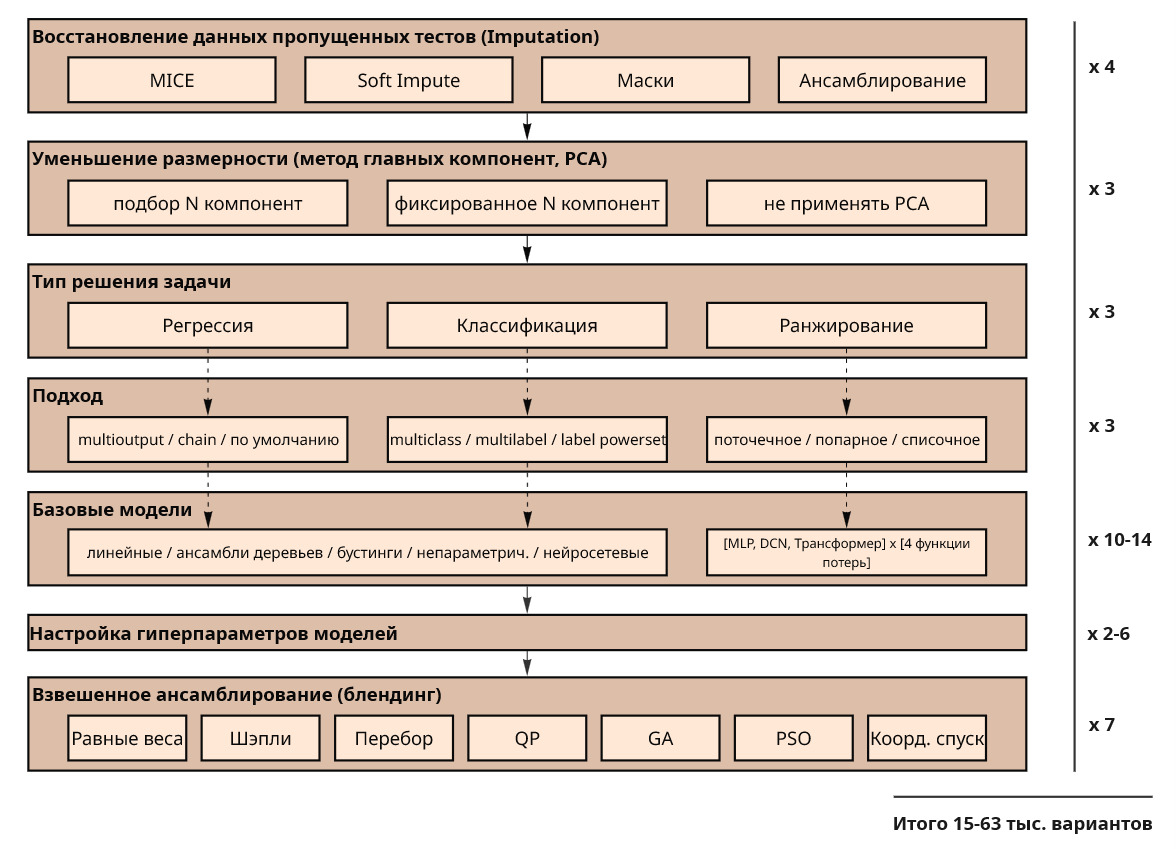
\includegraphics[width=1\linewidth]{figures/multi_pipeline.jpg}
    \caption{Общая схема вариантов экспериментального исследования}
    \label{fig:multi_pipeline}
\end{figure}

Общая схема вариантов экспериментального исследования представлена на  рисунке~\ref{fig:multi_pipeline}. Оценка каждого варианта проводится в соответствии с мерой сходства C-индекс. 

Следует отметить, что этап уменьшения размерности может:
\begin{itemize}[noitemsep, topsep=0pt, parsep=0pt, partopsep=0pt]
    \item[-] не выполняться вовсе;
    \item[-] применяться с фиксированным порогом на уровне 90\% объяснённой дисперсии;
    \item[-] выполняться с динамическим подбором числа компонент (N).
\end{itemize}
На этапе ранжирования поточечный и попарный подходы могут пропускаться в пользу списочного (\emph{listwise}). Конкретный выбор базовых моделей регрессии и классификации более подробно описан в разделах~\ref{subsec:regr} и~\ref{subsec:classif}. Для списочного ранжирования рассматриваются все возможные комбинации трёх архитектур (многослойный перцептрон, глубокая перекрёстная сеть, трансформер) и четырёх функций потерь (\textsc{ApproxNDCG}, \textsc{ListNet@1}, \textsc{ListNet@3}, \textsc{LambdaRank}). Каждая из базовых моделей также требует подбора гиперпараметров, например, числа ближайших соседей \textit{k} для модели kNN. Итоговое число вариантов для перебора и определения наилучшего способа предсказания кода Голланда может достигать 63 тысяч различных способов, что создаёт значительную вычислительную нагрузку.

% !TeX spellcheck = ru_RU
% !TEX root = vkr.tex

\section{Особенности реализации программного инструмента для определения профориентационных предпочтений}

В разделе приведены технические детали реализации проекта: используемые языки и библиотеки, описание набора данных, архитектура кода и ключевые функции для подготовки данных, построения и оценки моделей (регрессия, классификация, ранжирование, ансамблирование), а также структура прототипа веб-приложения на R Shiny.


\subsection{Общие особенности реализации}

Реализация моделей определения профориентационных предпочтений на основе психометрических тестов личности производилась на языке R (версия 4.4.2)\footnote{\quad R Core Team. \textit{R: A Language and Environment for Statistical Computing}. R Foundation for Statistical Computing, Vienna, Austria.~--- 2024. URL: \url{https://www.R-project.org/} (дата обращения: 17.05.2025).}, являющимся открытым и свободным программным обеспечением. Язык R обеспечивает эффективность обработки данных за счёт векторизованных операций и оптимизированных реализаций статистических алгоритмов в базовых и дополнительных пакетах. Для обработки данных преимущественно использовались библиотеки \emph{data.table} для эффективных табличных преобразований, \emph{tidyverse} (различные манипуляции с данными \emph{dplyr}, элементы функционального программирования с \emph{purrr}, работа со строками через \emph{stringr}), \emph{arrow} для передачи наборов данных между R и Python, визуализация в \emph{plotly}. Нейросетевые модели реализованы на языке Python (версия 3.12.3)\footnote{\quad Van Rossum G, Drake FL. Python 3 Reference Manual. Scotts Valley, CA: CreateSpace.~--- 2009.} с использованием открытого и свободного ПО: \emph{numpy} и \emph{pandas} для численных вычислений и подготовки данных, \emph{PyTorch} как гибкий фреймворк для построения и обучения глубоких нейронных сетей.

Исходный код всего проекта представлен в GitHub-репозитории\footnote{\quad GitHub: Предсказание кода Голланда (RIASEC) по результатам психометрических тестов личности. URL: \url{https://github.com/ExP98/Diploma_Holland} (дата обращения: 17.05.2025).}. В репозитории представлена программная реализация вычислительного эксперимента, представленного на рисунке~\ref{fig:multi_pipeline}. Далее будут описаны ключевые шаги эксперимента с упоминанием названий функций и используемых библиотек, однако описание кода не является исчерпывающим. Код на языке R написан в соответствии с руководством по стилю оформления кода \emph{Tidyverse Style Guide}\footnote{\quad Руководство по стилю оформления кода на языке R. Tidyverse Style Guide. URL: \url{https://style.tidyverse.org/} (дата обращения: 17.05.2025).}, что обеспечивает единообразие оформления, читаемость и простоту сопровождения.

Инструмент автоматизации процесса профориентации состоит из следующих модулей:
\begin{itemize}
    \item модуль обработки данных;
    \item модуль восстановления данных;
    \item модуль обучения базовых моделей;
    \item модуль формирования взвешенного ансамбля моделей;
    \item модуль организации и проведения вычислительных экспериментов.
\end{itemize}
Предварительно проводился разведочный анализ данных. По результатам вычислительного эксперимента происходил выбор наилучших подходов для определения кода Голланда, обучение и сохранение лучшей модели. На её основе реализуется прототип инструмента автоматизации профориентации: веб-приложение на основе R Shiny.


\subsection{Описание набора данных. Разведочный анализ}

Данные для исследования были собраны с помощью опросов, размещенных в веб-приложении на базе платформы VK Mini Apps \enquote{Психологические тесты}\footnote{\quad Мини-приложение \enquote{Психологические тесты} (платформа \enquote{VK Mini Apps}). URL: \url{https://vk.com/app7794698} (дата обращения: 17.05.2025).}~\cite{vk_psychotests}. Приложение находится в открытом доступе и позволяет пользователям проходить различные психометрические опросы, при этом после ознакомления с условиями добровольного информированного согласия\footnote{\quad Политика конфиденциальности. URL: \url{https://vk.com/@ticslabs-politika-konfidencialnosti} (дата обращения: 17.05.2025).} пользователи могут разрешить использовать обезличенные анонимизированные данные в научных исследованиях (в соответствии с №~152-ФЗ \enquote{О персональных данных}).

\begin{figure}[bhtp]
    \centering
    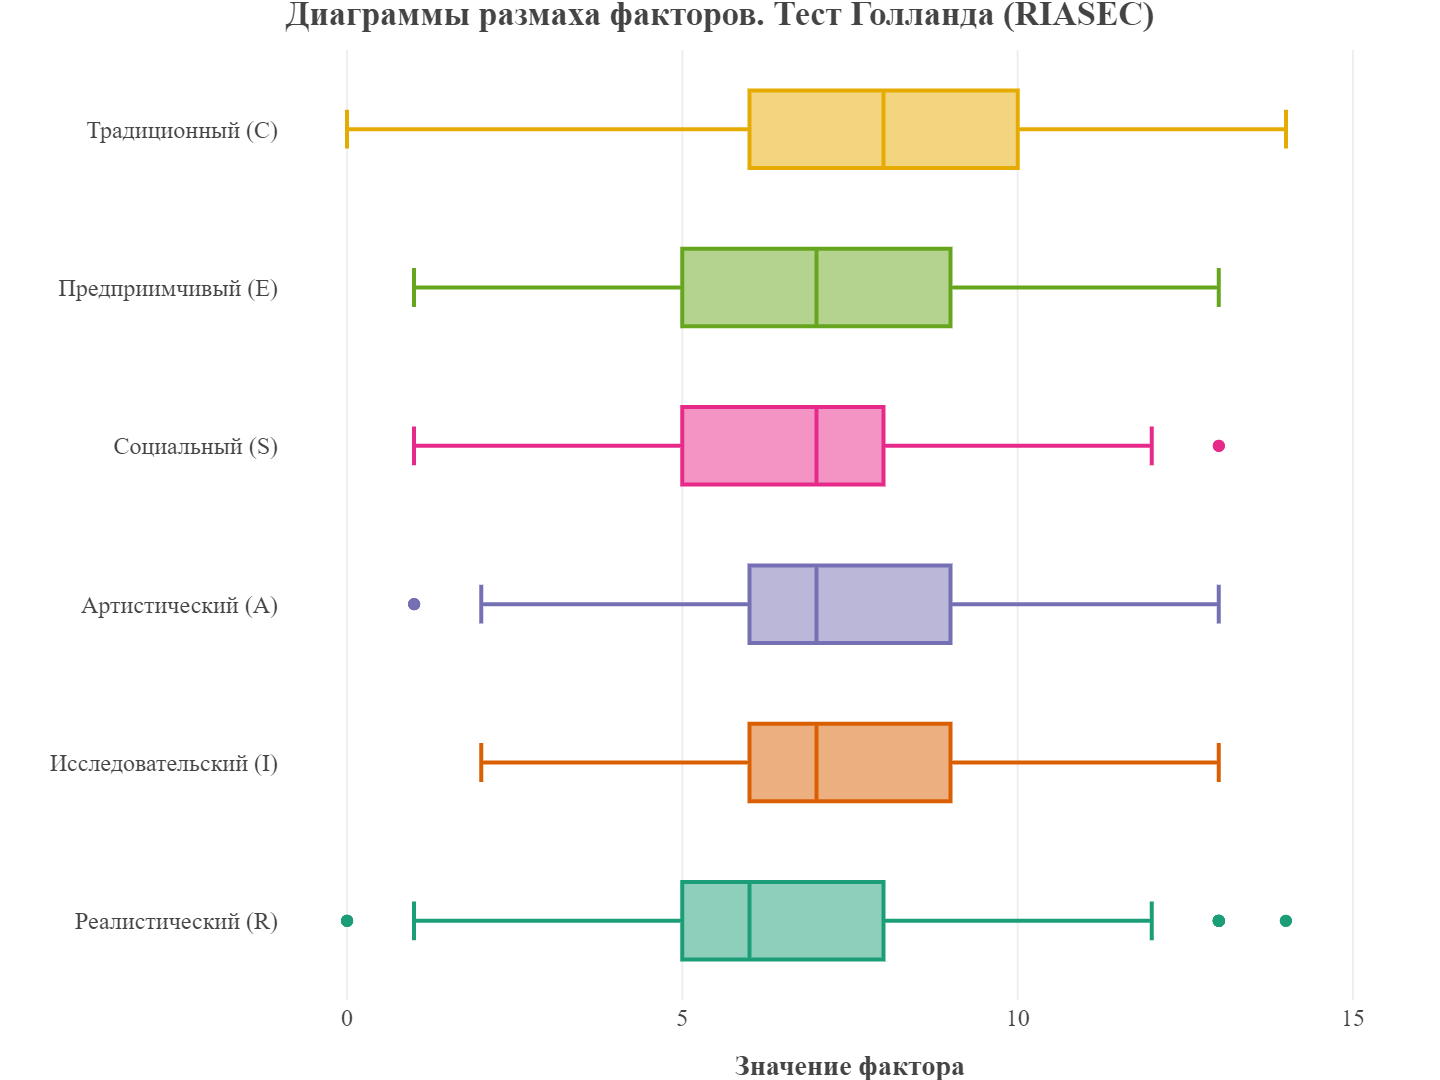
\includegraphics[width=0.75\linewidth]{figures/HL.png}
    \caption{Диаграмма размаха факторов модели Голланда}
    \label{fig:HL_boxplot}
\end{figure}

В наборе представлены данные по следующим психометрическим тестам (в скобках указано количество факторов):
\begin{enumerate}[noitemsep, topsep=4pt]
    \item Опросник Леонгарда-Шмишека (10).
    \item Личностный опросник Айзенка (4).
    \item 16-факторный опросник Кеттелла (16).
    \item Пятифакторный опросник личности (\enquote{Большая пятёрка}; 5).
    \item Ценностный опросник Шварца (20).
\end{enumerate}
Более подробное описание тестов и их факторов представлено в подразделе~\ref{sec:psytests}. Всего имеются данные по 1278 пользователям: у 339 есть данные по всем тестам, у 939 пользователей отсутствует один или два теста. Пример части преобразованного набора данных представлен в таблице~\ref{tab:input_test_data}. Диаграмма размаха для факторов модели Голланда представлена на рисунке~\ref{fig:HL_boxplot}, плотность их фактических значений~--- на рисунке~\ref{fig:facet}, частоты значений кодов в порядке убывания их значимости~--- рисунок~\ref{fig:ranks}. 

\begin{figure}[bhtp]
    \centering
    \begin{minipage}[b]{0.49\linewidth}
        \centering
        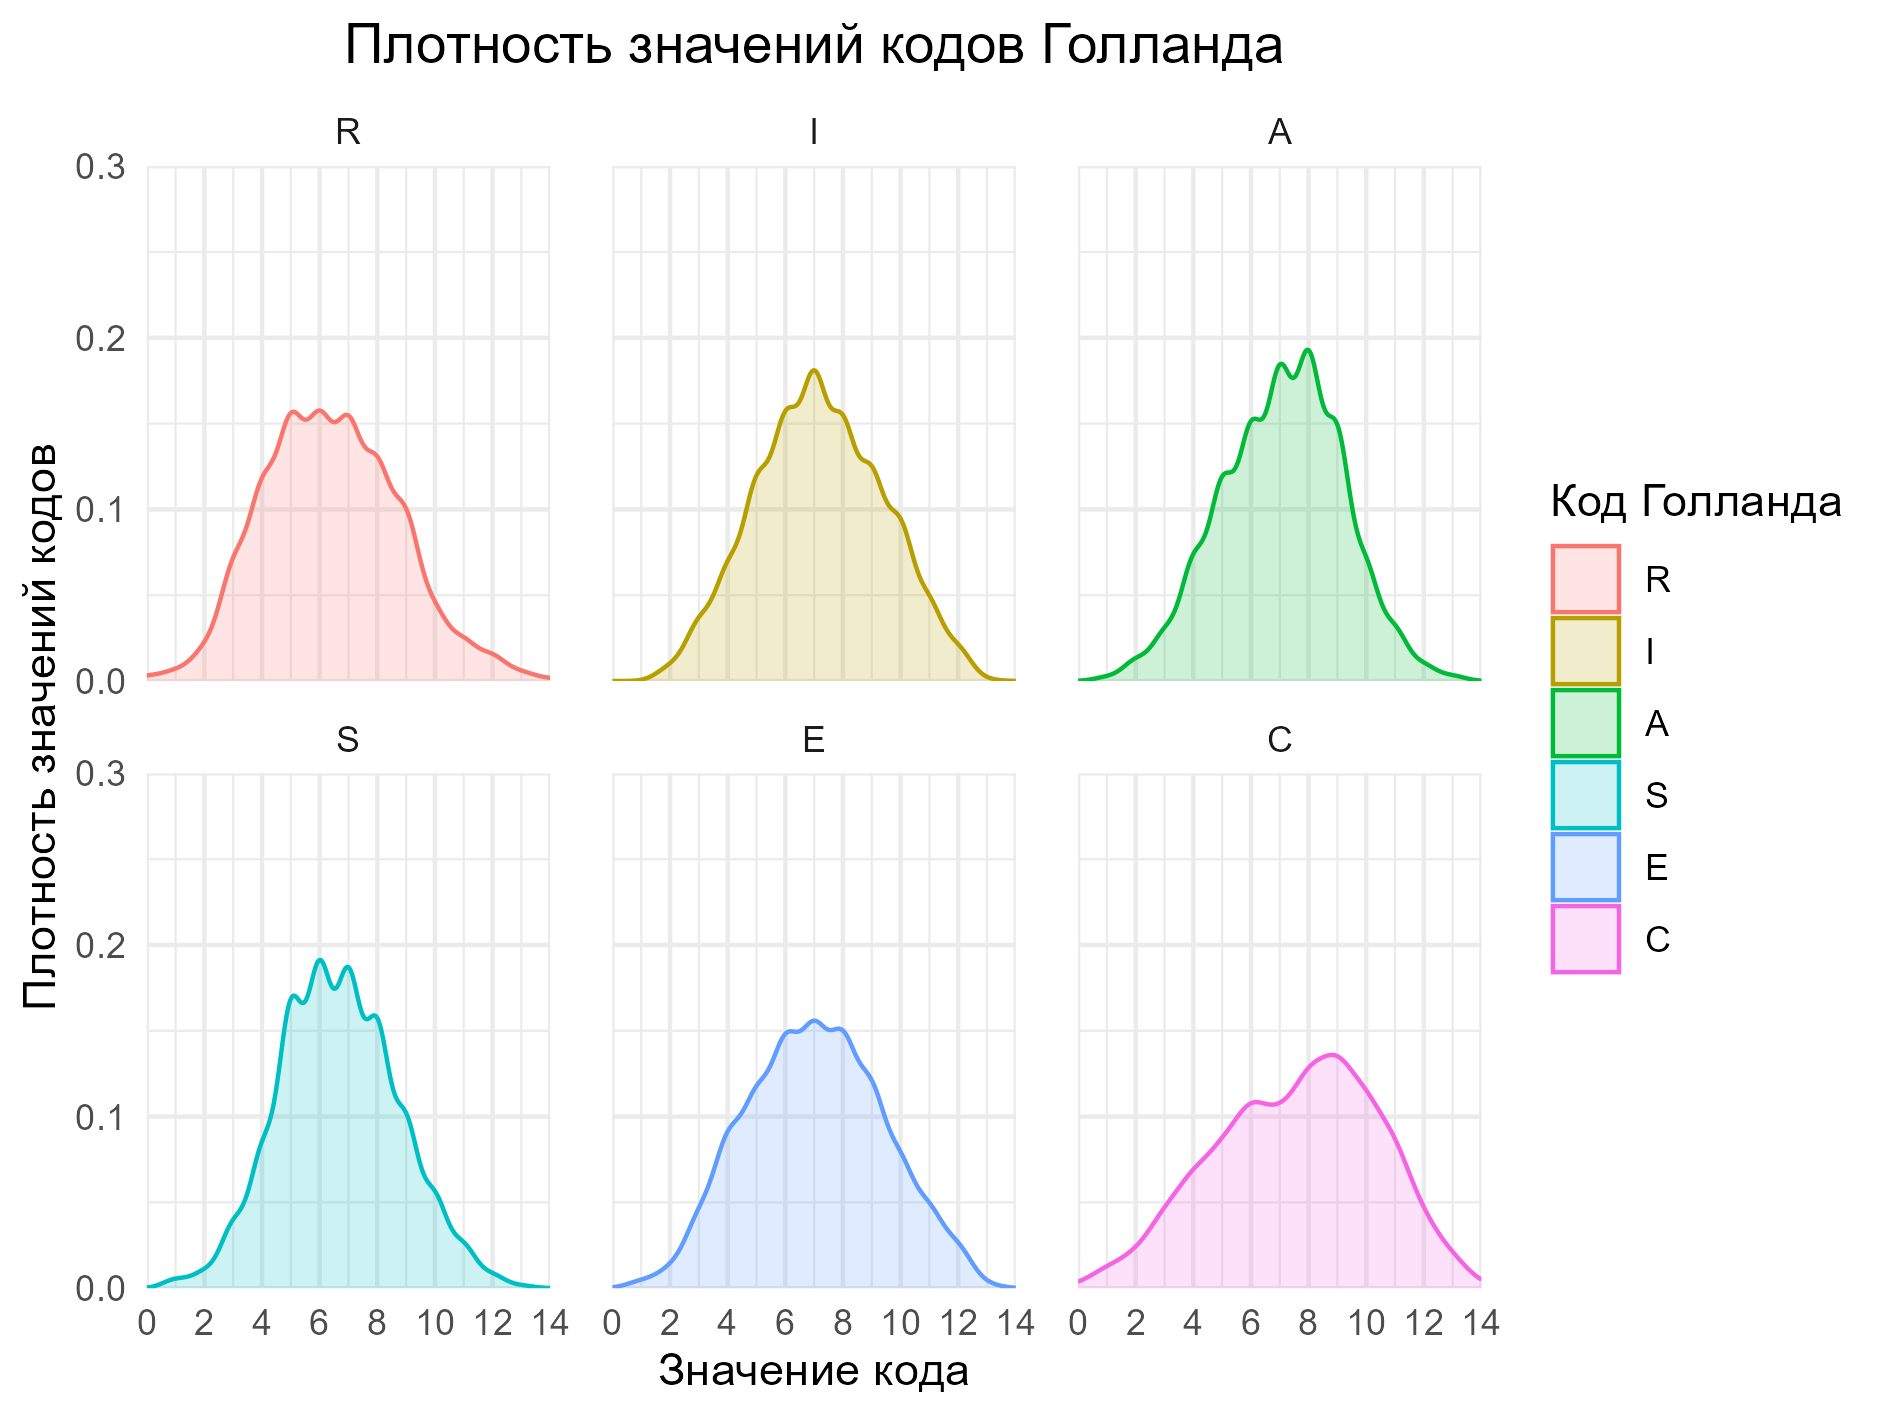
\includegraphics[width=\linewidth]{figures/facet.png}
        \caption{Плотность фактических значений кодов Голланда}
        \label{fig:facet}
    \end{minipage}
    \hfill
    \begin{minipage}[b]{0.49\linewidth}
        \centering
        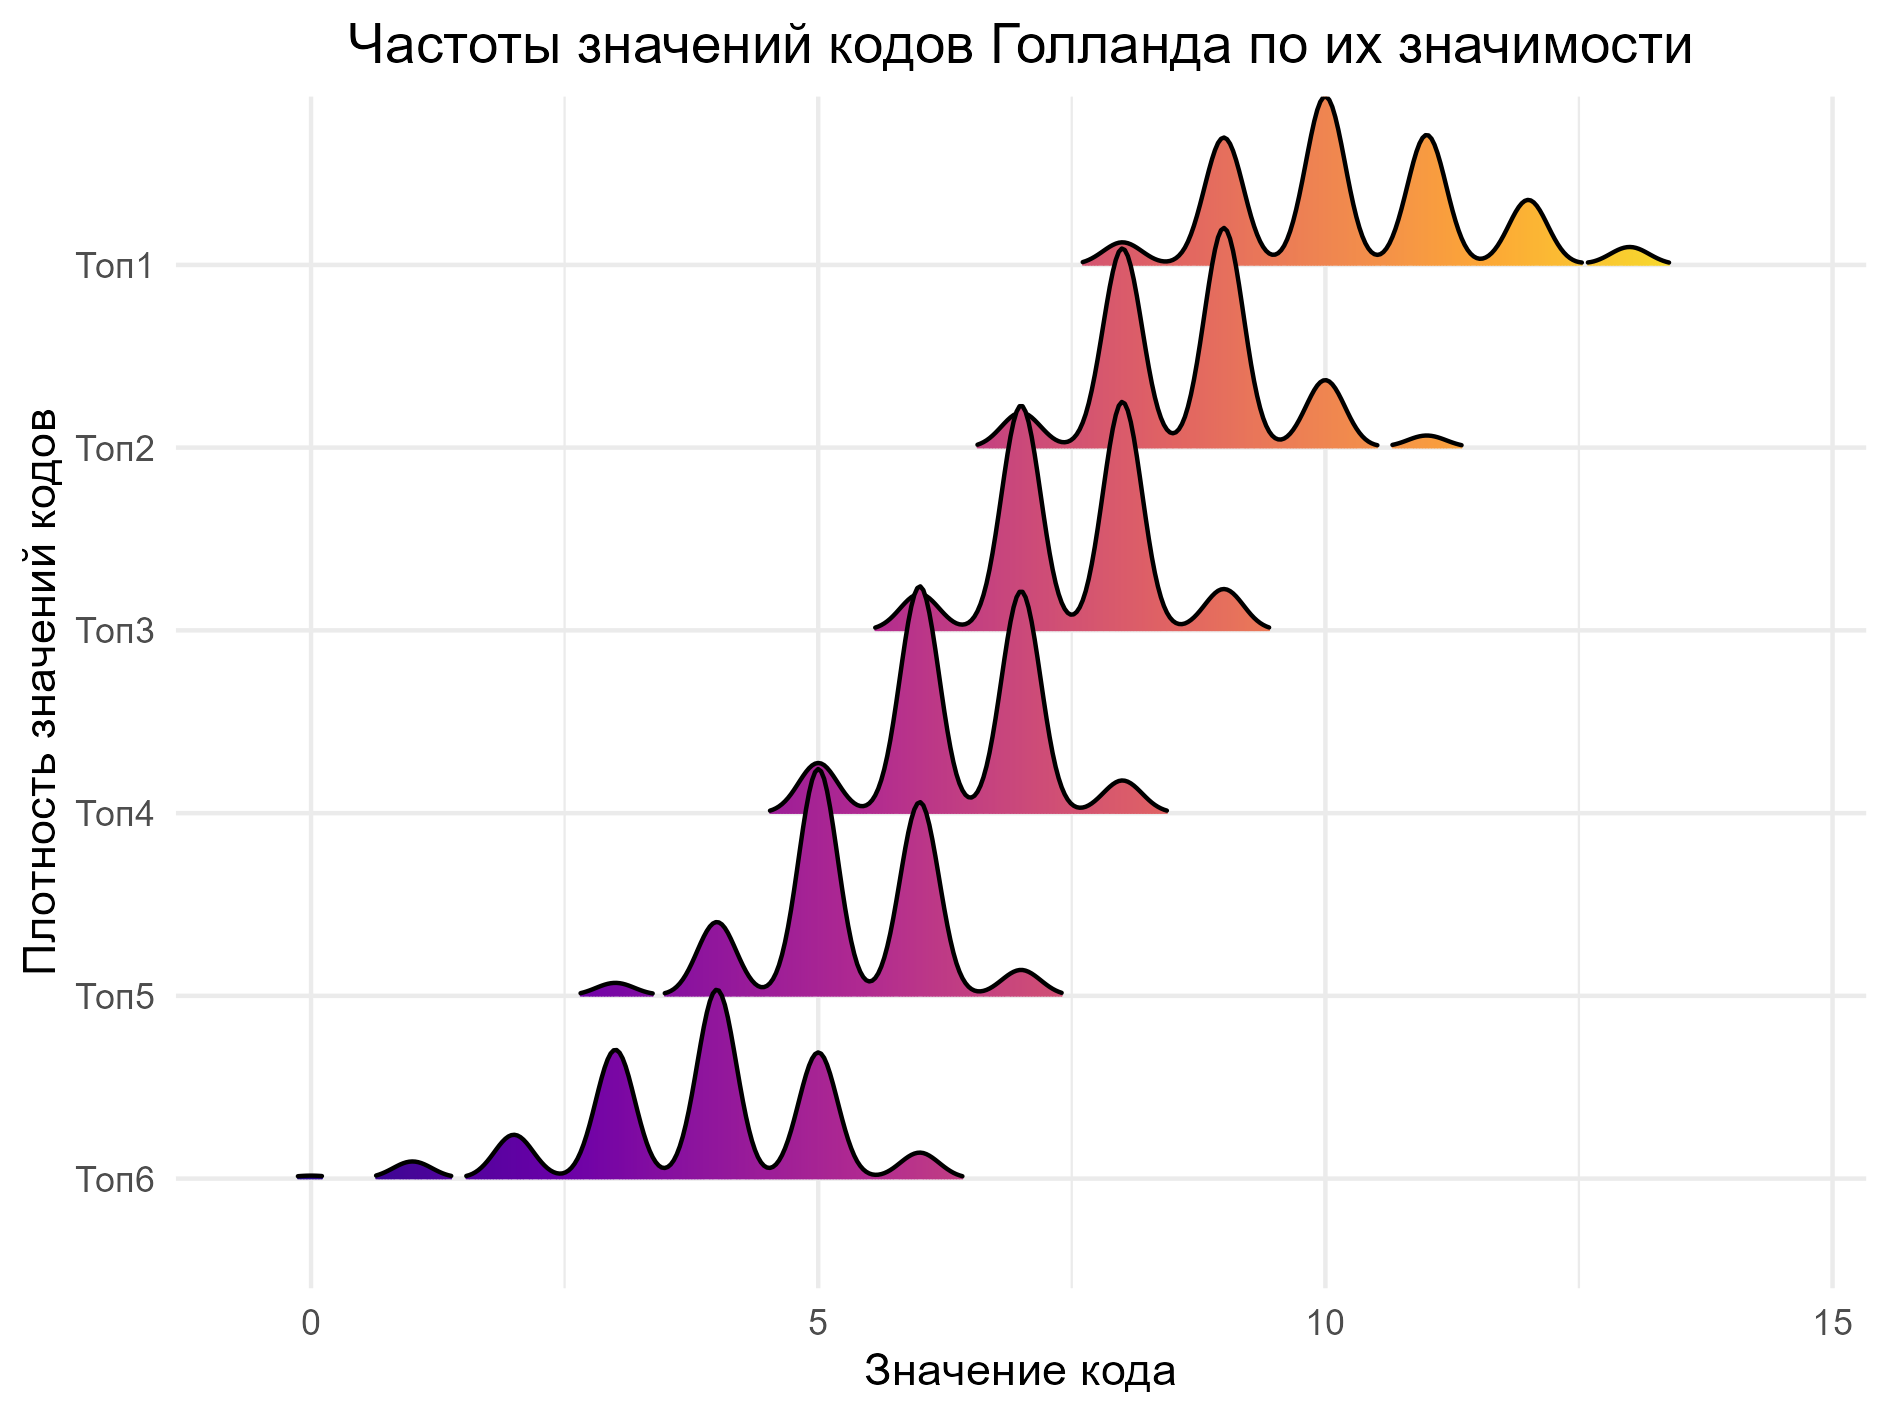
\includegraphics[width=\linewidth]{figures/ranks.png}
        \caption{Частоты значений кодов Голланда в порядке убывания их значимости}
        \label{fig:ranks}
    \end{minipage}
\end{figure}

Для анализа линейных связей между факторами модели Голланда на рисунке~\ref{fig:HL_cor} приведена матрица корреляций: коэффициент корреляции Пирсона по модулю не превышает $0.4$ (умереннная зависимость). Описательная статистика по всем факторам всех психометрических тестов приведена в Приложении~\ref{app:psytests} в таблице~\ref{tab:psytests_desc_stats}. Каждый из представленных факторов является числовой метрической переменной, принимающей только целочисленные значения.

\begin{figure}[bhtp]
    \centering
    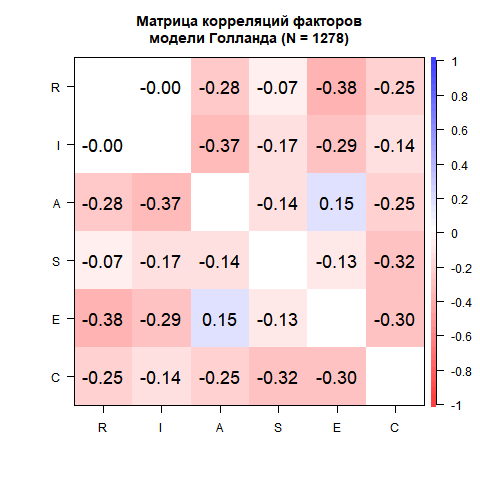
\includegraphics[width=0.6\linewidth]{figures/cor_united.png}
    \caption{Матрица корреляций кодов Голланда}
    \label{fig:HL_cor}
\end{figure}

К основным ограничениям исследования относятся особенности сбора данных: возможны смещения из-за специфики портала, а также способа формирования выборки. Для устранения ограничений может быть увеличен размер выборки, включены вопросы о социально-демографических признаках опрашиваемых.


\subsection{Особенности реализации модулей программного инструмента}

\subsubsection{Модуль обработки и восстановления данных}

Данные по пройденным пользователями тестам были получены в json-формате, где пользователю поставлен в соответствие пройденный им тест с результатами. Данные были преобразованы в \enquote{широкий} табличный формат, заполнены самоочевидные пропуски (исходя из природы психометрических данных), проведена валидация данных в соответствии с допустимыми значениями каждого из факторов психометрических тестов. Для проведения вычислительного эксперимента данные были поделены на обучающую, валидационную и тестовую выборки. Нормализация (стандартизация) данных всех выборок происходит в соответствии со средним значением и с значением стандартного отклонения, вычисляемым по обучающей выборке (функции \lstinline{transform_data_to_wide}, \lstinline{train_test_split} в программном коде).

Уменьшение размерности было реализовано в виде метода главных компонент (PCA) с помощью библиотеки \emph{stats}, функции \lstinline{prcomp}. В результате набора экспериментов было найдено, что чаще всего наилучший результат обеспечивает снижение размерности до 90\% объясняемой дисперсии, а именно до 30 компонент; таким образом, сравнение моделей велось и на полном наборе данных, и на данных меньшей размерности ($N_{comp} = 30$). В дальнейшем для моделей (если не указано иное) итоговое значение метрики~--- это лучшее из значений метрики модели на полном наборе данных и на наборе меньшей размерности.

Восстановление значений факторов незаполненных психометрических тестов для множественной импутации реализовано в функции \lstinline{mice_imputation} (в основе лежит реализация из библиотеки \emph{mice}); низко\-ранговая матричная аппрокси\-мация (\mbox{листинг}~\ref{lst:softimpute})~--- \lstinline{train_matrix_completion} для учета зависимостей и \lstinline{transform_matrix_completion} для преобразования с использованием библиотеки \emph{softImpute}; \lstinline{prepare_mask_data} для применения масок.

\begin{listing}
    \caption{Низкоранговая матричная аппроксимация \emph{Soft Impute}}
    \label{lst:softimpute}
    \begin{minted}[frame=lines]{r}
train_matrix_completion <- function(DT, rank.max = 20) {
  aux_feats <- setdiff(colnames(DT), c("id", paste0("HL_", 1:6)))
  M         <- as.matrix(DT)[, aux_feats]
  fit       <- softImpute::softImpute(M, rank.max = rank.max, lambda = 0, type = "als")
  return(list(fit = fit, aux = aux_feats))
}

transform_matrix_completion <- function(fit_obj, DT_new) {
  DT_new <- DT_new %>% as.matrix() %>%
    softImpute::complete(fit_obj$fit) %>%
    {DT_new[, fit_obj$aux] <- .; DT_new}
  return(DT_new)
}
  \end{minted}
\end{listing}


\subsubsection{Модуль обучения базовых моделей}

Базовые модели регрессии и классификации, перечисленные в подразделах~\ref{subsec:regr} и~\ref{subsec:classif}, в языке R реализованы в различных пакетах: линейная регрессия (\emph{lm}) в пакете \emph{stats}, регуляризованная регрессия~--- \emph{glmnet}, пошаговая~--- \emph{MASS}; одноимённые модели в пакетах \emph{xgboost}, \emph{lightgbm}, \emph{catboost}, \emph{randomForest}; метод k-ближайших соседей в \emph{FNN} и \emph{caret}; метод опорных векторов и наивный байесовский классификатор в \emph{e1071}; алгоритм ExtraTrees в \emph{ranger}. Для проведения экспериментов разработан унифицированный интерфейс взаимодействия с моделями: с помощью пакета \emph{R6} реализованы соответствующие классы-обёртки, наследующие шаблонный класс \lstinline{my_template_model}, в которых при необходимости переопределены методы \lstinline{initialize()}, \lstinline{fit()} и \lstinline{predict()}. Многие модели, например, случайный лес, бустинги, линейные регрессии, позволяют вычислять важность признаков, поэтому для них определен метод \lstinline{calc_importance()}.

Для решения задачи регрессии с помощью нейронных сетей был взят язык \emph{Python} и фреймворк \emph{PyTorch}. Первая модель из трёх реализованных представляет собой простой многослойный перцептрон с четырьмя плотными слоями ($55 \rightarrow 128 \rightarrow 64 \rightarrow 32 \rightarrow 6$) и функцией активации ReLU: такое снижение размерности позволяет постепенно выделять всё более абстрактные признаки из исходных 55 факторов и сразу выдавать шесть прогнозируемых значений. Вторая модель расширена модулями нормализации (BatchNorm) и регуляризации (Dropout, L1/L2-регуляризация, весовой спад) на каждом скрытом слое, что улучшает сходимость, устойчивость к переобучению и ускоряет обучение: сочетание таких приёмов и глубины должно обеспечивать баланс между выразительностью сети и её обобщающей способностью. В качестве третьей модели используется \emph{TabPFN} (библиотека \emph{tabpfn})~--- это трансформер, предобученный на большом числе синтетических табличных задач и предлагающий встроенную байесовскую оценку неопределённости. Он позволяет мгновенно делать предсказания без итеративного обучения, автоматически адаптируясь к различным типам признаков и небольшим объёмам данных. Модель \emph{TabPFN} также демонстрирует стабильные результаты в условиях разнородных и зашумлённых данных.

Решение задачи ранжирования также было реализовано в \emph{Python} с помощью \emph{PyTorch} (подклассы \lstinline{nn.Module}). Для списочного ранжирования были реализованы три класса:
\begin{itemize}
    \item \lstinline{MLPRanker} включает четыре полносвязных слоя размерности [$55 \rightarrow 128 \rightarrow 64 \rightarrow 32 \rightarrow 6$] с последовательным применением BatchNorm и Dropout. Такая глубина позволяет постепенно снижать размерность признаков и выделять всё более абстрактные комбинации без избыточного роста числа параметров.
    \item \lstinline{DCNUserItemRanker} сочетает три перекрёстных (\emph{cross}) слоя, моделирующих полиномиальные взаимодействия входных признаков, и \enquote{глубокую} ветвь из линейных блоков [$64 \rightarrow 128 \rightarrow 64 \rightarrow 32$] с ReLU и Dropout. Число перекрёстных слоёв выбрано эмпирически: трёх итераций перекрёстных преобразований достаточно для учёта основных взаимодействий, при этом обучение остаётся устойчивым.
    \item Модель \lstinline{ListwiseTransformer} для каждого из шести элементов создаёт обучаемое представление (эмбеддинг) размерности 8, объединяет его с 55-мерным входным вектором, затем проецирует результат в пространство размерности 64 (\lstinline{d_model = 64}). Далее он проходит через два слоя кодировщика на основе трансформера с четырьмя головами внимания (\lstinline{nhead = 4}) и завершается одним линейным выходным слоем. Использование двух слоёв обеспечивает баланс между учётом взаимного влияния элементов и приемлемым временем обучения.
\end{itemize}
Каждый из классов комбинируется с четырьмя функциями ошибок, соответствующих списочной оптимизации:
\begin{itemize}
    \item \lstinline{ListNet@1} и \lstinline{ListNet@3} вычисляют кросс-энтропию между распределениями рангов (полным или усечённым до топ-3) с помощью функции \lstinline{softmax};
    \item \lstinline{ApproxNDCG} аппроксимирует классическую метрику NDCG, вводя дифференцируемые ранги через сигмоидные функции;
    \item \lstinline{LambdaRank} формирует парно-ориентированную функцию ошибок с расчётом $\lambda$-коэффициентов на основе $\Delta\mathrm{NDCG}$ при перестановках.
\end{itemize}

\begin{listing}
    \caption{Функция подсчета важности моделей на основе вектора Шэпли (с применением стохастического метода Монте-Карло)}
    \label{lst:weight_optim_shap}
    \begin{minted}[frame=lines]{r}
approx_shapley <- function(models_probs, Y_true, R = 500) {
  M <- length(models_probs)
  prob_array <- simplify2array(models_probs)
  phi <- numeric(M)
  for (r in seq_len(R)) {
    perm <- sample.int(M)
    cum_sum <- 0
    v_prev <- 0
    for (k in seq_along(perm)) {
      idx <- perm[k]
      cum_sum <- cum_sum + prob_array[,, idx]
      v_curr <- matr_cind(cum_sum / k, Y_true)
      phi[idx] <- phi[idx] + (v_curr - v_prev)
      v_prev <- v_curr
    }
  }
  w <- phi / R
  return(w / sum(w))
}
  \end{minted}
\end{listing}


\subsubsection{Модуль формирования взвешенного ансамбля моделей}

Подбор весов моделей для дальнейшего взвешенного ансамблирования (линейного блендинга) был реализован в следующих функциях:
\begin{itemize}
    \item равные веса всех моделей~--- функция \lstinline{equal_weights};
    \item вектор Шэпли~--- \lstinline{approx_shapley} (листинг~\ref{lst:weight_optim_shap}). Для ускорения работы функции производилась стохастическая аппроксимация с использованием метода Монте-Карло: вместо полного перебора всех вариантов были выбраны \emph{R} перестановок (разброс значений оценок уменьшается пропорционально $1/\sqrt{R}$);
    \item частичный перебор по сетке~--- \lstinline{grid_search_weights} с заданием шага сетки;
    \item квадратичная оптимизация в функции \lstinline{stacking_qp_weights}, использующая функцию \lstinline{solve.QP} библиотеки \emph{quadprog};
    \item генетический алгоритм и метод роя частиц~--- реализованы на основе функций \lstinline{ga} библиотеки \emph{GA} и \lstinline{psoptim} из \emph{PSO} (код функции \lstinline{particle_swarm_weights} приведен в листинге~\ref{lst:weight_optim_pso});
    \item координатный спуск~--- функция \lstinline{coordinate_optimize_weights} (использует библиотеку \emph{stats}).
\end{itemize}

От использования подбора весов с помощью байесовской оптимизации (библиотека \emph{rBayesianOptimization}) было решено отказаться вследствие больших вычислительных затрат (разница во времени выполнения, например, с методом роя частиц в два порядка).

Таким образом, способы подбора весов были реализованы как собственными средствами, так и с использованием возможностей, встроенных в различные пакеты.

\begin{listing}
    \caption{Функция подсчета важности моделей на основе метода роя частиц (PSO)}
    \label{lst:weight_optim_pso}
    \begin{minted}[frame=lines]{r}
particle_swarm_weights <- function(models_probs, Y_true, swarm_size = 50, maxit = 100) {
  M <- length(models_probs)
  fn_pso <- function(x) {-weighted_cindex_value(x / sum(x), models_probs, Y_true)}
  PSOres <- pso::psoptim(par = rep(1/M, M), fn = fn_pso, lower = rep(.Machine$double.eps, M), upper = rep(1, M), control = list(s = swarm_size, maxit = maxit, trace = FALSE, vectorize = TRUE, maxit.stagnate = 10))
  w <- PSOres$par
  w[w < 1e-6] <- 0
  return(w / sum(w))
}
  \end{minted}
\end{listing}


\subsubsection{Модуль организации и проведения вычислительных экспериментов}

При разработке решения задачи многоцелевой регрессии были реализованы походы независимого предсказания выходов (значений кодов Голланда) \lstinline{stack_MO_regr}, предсказаний по цепочке \lstinline{chain_MO_regr} и \lstinline{no_MO_regr} для предсказаний моделей, поддерживающих множественные выходы по умолчанию. Наличие унифицированных интерфейсов (R6-классов) с базовыми моделями позволило организовать массовую оценку моделей с помощью функции \lstinline{calc_regression_models}, на вход которой подается следующий набор данных: название класса модели, её метка и гиперпараметры, подход к многоцелевой регрессии; код представлен в листинге~\ref{lst:calc_regr}. Аналогичный подход был использован для реализации подходов к решению задачи классификации: на основе унифицированной функции-интерфейса \lstinline{classification_test_framework}, позволяющего обучить модель, сделать предсказание, оценить значения метрик качества (C-индекс и точность Top-K), применяется функция, например, \lstinline{run_multilabel_experiments} для многометочной классификации (листинг~\ref{lst:multilabel_clsf}).

\begin{listing}
    \caption{Функция массовой оценки регрессионных моделей}
    \label{lst:calc_regr}
    \begin{minted}[frame=lines]{r}
calc_regression_models <- function(regr_models_df, X_train_, Y_train_, X_test_, Y_test_) {
  MO_res <- regr_models_df %>% 
    copy() %>% 
    .[, pred := pmap(list(model, params, MO_type), \(mdl, par, mo_type) do.call(perform_MO_regression, 
        c(list(mdl, mo_type, X_train_, Y_train_, X_test_, Y_test_, print_model_name = F), par)))] %>% 
    .[, rmse := map_dbl(pred, \(x) df_metric(x, Y_test_, my_rmse) %>% round(3))] %>% 
    .[map_lgl(pred, \(item) !is.null(item)),
      C_index := map_dbl(pred, \(x) df_metric(x, Y_test_, calc_C_index) %>% round(3))] %>% 
    .[, .(name, pred, rmse, C_index)]
  return(MO_res)
}
  \end{minted}
\end{listing}

\begin{listing}
    \caption{Функция массовой оценки решения задачи многометочной классификации}
    \label{lst:multilabel_clsf}
    \begin{minted}[frame=lines]{r}
run_multilabel_experiments <- function(experiments_df, X_train, Y_b_train, 
                                       X_test, Y_b_test) {
  # experiments_df (tibble/data.table): clsf_func, label, params, n_retry
  evaluate_ML <- function(multlbl_clsf_func, label = "", n_retry = 1, ...) {
    classification_test_framework(Y_test = Y_b_test, Y_b_test = Y_b_test, 
                                  clsf_func = multlbl_clsf_func, n_retry = n_retry, 
                                  label = label, X_train = X_train, 
                                  Y_b_train = Y_b_train, X_test = X_test, ...)
  }
  
  res <- experiments_df %>%
    as.data.table() %>%
    .[, metrics := pmap(list(multlbl_clsf_func, label, params, n_retry), \(ind_fn, lbl, extra_args, nr) 
                        do.call(evaluate_ML, c(list(multlbl_clsf_func = ind_fn, label = lbl, n_retry = nr), extra_args))
    )] %>%
    .[, .(label, metrics, id = 1:.N)] %>%
    .[, metrics[[1]], by = id]
  
  return(res)
}
  \end{minted}
\end{listing}


\subsection{Реализация прототипа инструмента для определения профориентационных предпочтений}

Прототип инструмента для определения профориентационных предпочтений был реализован в виде интерактивного веб-приложения на платформе R Shiny. На рисунке~\ref{fig:pipeline} приведён общий порядок вычислительного конвейера разработанного прототипа программного инструмента, в котором последовательно выполняются все необходимые шаги: от предобработки и очистки исходных данных до восстановления пропусков с помощью модели мягкого матричного восстановления \emph{Soft Impute} и дальнейшего прогнозирования с помощью предварительно обученной и сохраненной модели регуляризованной L1-регрессии (\emph{Lasso}), показавшей наилучшие результаты среди базовых моделей (при оценке C-индекса).

\begin{figure}[htbp]
    \centering
    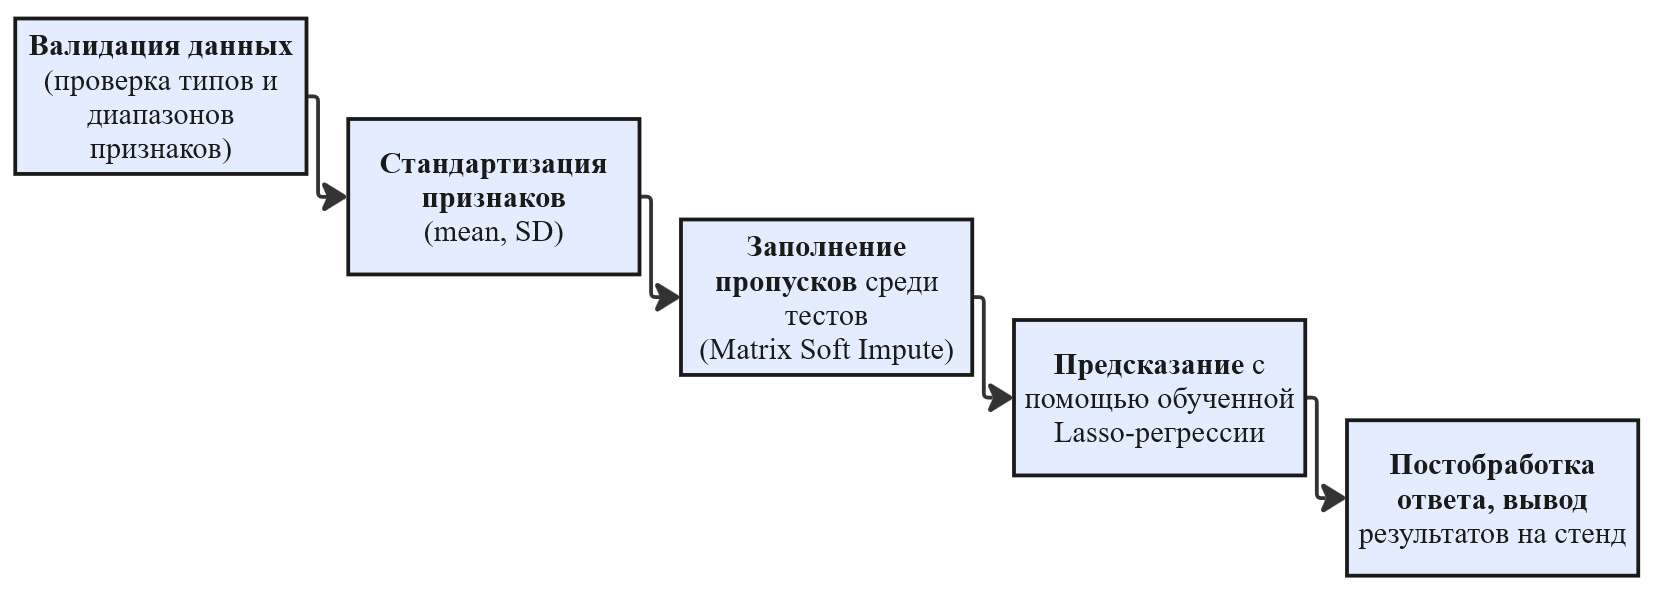
\includegraphics[width=1.0\linewidth]{figures/final_pipeline.jpg}
    \caption{Итоговая последовательность вычислительных шагов}
    \label{fig:pipeline}
\end{figure}

При разработке веб-стенда на R Shiny в блоке кода \lstinline{ui} через \lstinline{fluidPage} и \lstinline{bsCollapse} с помощью функции \lstinline{create_test_ui} динамически формируется панель тестов с групповыми сворачивающимися блоками вопросов. В серверной части с помощью \lstinline{reactiveValues} для хранения промежуточных данных и \texttt{observeEvent(input\$calc)} организована реактивная логика: при нажатии \enquote{Подсчитать} происходит валидация входных значений (в случае выхода за рамки допустимых значений пользователю выводится сообщение об ошибке), восстановление пропусков методом \emph{Soft Impute} и нормализация данных, затем вызывается функция предсказания, а результаты выводятся через \lstinline{renderUI} и подтверждаются уведомлениями \lstinline{showNotification}. По завершении вычислений результаты в виде набора кодов рекомендуемых направлений сопровождаются подробным текстовым описанием и визуальной презентацией на пользовательском интерфейсе (см. интерфейс стенда на рисунках~\ref{fig:ui} и~\ref{fig:ui2}). Разделение на \lstinline{ui} и \lstinline{server} типично для \emph{Shiny}-приложений: \lstinline{ui} описывает компоненты интерфейса, а сервер~--- реактивную логику и обновление данных. Такой подход обеспечивает раздельную ответственность за внешний вид и вычислительную логику прототипа.

Доступ к приложению не требует процедуры авторизации, при этом его развертывание возможно как в локальной среде, так и на удалённом сервере с использованием средств хостинга. Разработанный прототип может быть использован в составе более комплексных информационных систем, направленных на поддержку профессиональной ориентации и образовательного планирования.

\begin{figure}[htbp]
    \centering
    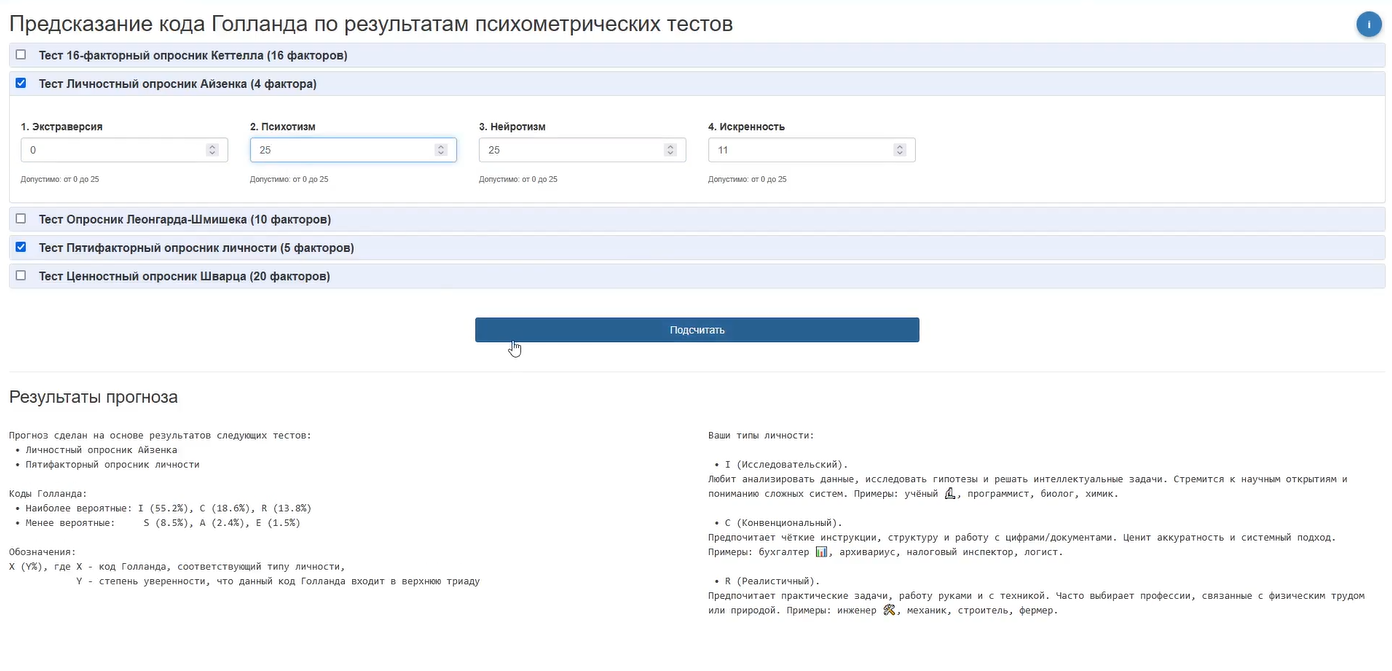
\includegraphics[width=1.0\linewidth]{figures/UI1.png}
    \caption{Интерфейс прототипа инструмента профориентации}
    \label{fig:ui}
\end{figure}


\clearpage
% !TeX spellcheck = ru_RU
% !TEX root = vkr.tex

\section{Результаты вычислительного эксперимента по определению кода Голланда}

\subsection{Сравнение результатов моделей на полных данных}

Для обеспечения сравнимости различных подходов (регрессия, классификация, ранжирование) между собой основное внимание было уделено мере сходства C-индекс (более подробное описание в подразделе~\ref{subsec:cindex}; чем выше значение, тем лучше; значение для случайного константного предсказателя равно $9.0$). Такой выбор меры позволяет сравнивать результаты с другими научными работами. Так, на основе социо-демографических данных в работе~\cite{Bogacheva} достигается значение $\text{C‑index}~=~10.95$ для регрессии и $\text{C‑index}~=~11.08$ для классификации, поэтому результат предсказания с таким же значением или больше может считаться приемлемым.

\begin{table}[!ht]
  \centering
  \caption{Сравнение регрессионных моделей, C‑индекс}
  \label{tab:regr_res}
    \setlength{\tabcolsep}{2pt}
    \begin{tabular*}{\textwidth}{@{\extracolsep{\fill}} 
      >{\raggedright\arraybackslash}m{6.25cm}  
      | *{4}{>{\centering\arraybackslash}m{2.35cm}}
    @{}}
  \toprule
      \textbf{Модель} 
        & \textbf{Multi\-output}      
        & \textbf{Мult. PCA}   
        & \textbf{Chain}   
        & \textbf{Chain PCA} \\
    \midrule
    Регрессия Lasso (L1)      & \g{11.175} & \g{10.887} & \g{11.175} & \g{11.150} \\
    ExtraTrees                & \g{10.700} & \g{11.100} & \g{10.625} & \g{10.825} \\
    Регрессия Ridge (L2)      & \g{10.988} & \g{10.537} & \g{11.062} & \g{10.412} \\

    \arrayrulecolor[gray]{0.8}
    \specialrule{0.75pt}{0pt}{0pt}
    \arrayrulecolor{black}
    
    Метод опорных векторов    & \g{10.713} & \g{10.950} & \g{10.713} & \g{10.950} \\
    Пошаговая регрессия       & \g{10.605} & \g{10.905} & \g{10.600} & \g{10.905} \\
    CatBoost                  & \g{10.688} & \g{10.812} & \g{10.688} & \g{10.812} \\
    Случайный лес             & \g{10.625} & \g{10.475} & \g{10.812} & \g{10.588} \\
    Линейная регрессия (OLS)  & \g{10.688} & \g{10.800} & \g{10.688} & \g{10.800} \\
    LightGBM                  & \g{10.750} & \g{10.425} & \g{10.750} & \g{10.425} \\
    kNN                       & \g{10.525} & \g{10.400} & \g{10.525} & \g{10.400} \\
    XGBoost                   & \g{9.164}  & \g{9.729}  & \g{9.162}  & \g{9.725}  \\
    Constant baseline         & \g{9.000}  & \g{9.000}  & \g{9.000}  & \g{9.000}  \\
    \midrule
    TabPFN                    & \g{10.562} &            &            &            \\
    MLP (BatchNorm, DropOut, регуляризация) & \g{10.462} &    &            &            \\
    MLP                       & \g{10.275} &            &            &            \\
    \bottomrule
  \end{tabular*}
  \vspace{0.75em}
  \begin{minipage}{\textwidth}
      \small
      \textit{Обозначения:\\
      \hspace*{1em}Mult.~--- multioutput, предсказание переменных независимо друг от друга,\\
      \hspace*{1em}Chain~--- предсказание выходных переменных по цепочке,\\
      \hspace*{1em}PCA~--- метод главных компонент (уменьшение размерности)}
  \end{minipage}
\end{table}

\begingroup
\fontsize{7pt}{8pt}\selectfont
\begin{table}
  \centering
  \caption{Важность признаков модели случайного леса}
  \label{tab:feature_imp}
  \begin{tabular*}{\textwidth}{@{\extracolsep{\fill}} 
      >{\centering\arraybackslash}p{2.25cm}|
      >{\raggedright\arraybackslash}p{9cm}|c c @{}}
    \toprule
    \makecell{Код\\признака} 
      & \makecell[c]{Наименование признака} 
      & \makecell{Важность\\(\%)} 
      & \makecell{Накоплено\\(\%)} \\
    \midrule
    CT\_1   & Открытость--замкнутость                & 15.5 & 15.5 \\
    CT\_7   & Чувственность--твердость               & 15.5 & 31.0 \\
    SC\_19  & Гедонизм--индивидуальный приоритет     & 4.2  & 35.2 \\
    EY\_1   & Экстраверсия                           & 4.0  & 39.2 \\
    CT\_4   & Беспечность--озабоченность             & 3.6  & 42.8 \\
    SC\_3   & Власть--нормативный идеал              & 3.4  & 46.2 \\
    LN\_3   & Циклотимность                          & 3.3  & 49.5 \\
    BF\_3   & Самоконтроль--импульсивность           & 2.5  & 52.0 \\
    BF\_4   & Эмоц. устойчивость--неустойчивость     & 2.5  & 54.5 \\
    \bottomrule
  \end{tabular*}
\end{table}
\endgroup


Результаты определения кода Голланда как задачи регрессии (на основе C-индекса) приведены в таблице~\ref{tab:regr_res}. В сравнении с константным предсказателем модель XGBoost показывает низкие результаты. Наилучшие результаты показывает регуляризованная регрессия (Lasso и Ridge): $\text{C‑index}~=~11.175$ и $\text{C‑index}~=~11.062$. Высокий результат показывает модель ExtraTrees: $\text{C‑index}~=~11.1$. Лучшая из нейросетевых моделей, foundation-модель TabPFN, $\text{C‑index}~=~10.562$, показывает результат лучше лишь XGBoost и на одном уровне с методом k-ближайших соседей. Стоит отметить, что результаты моделей при различных подходах, независимом и по цепочке (\emph{multioutput} и \emph{chain}), практически идентичны. В то же время попарно для каждого из подходов лучшие результаты многие модели показывают на наборе данных меньшей размерности (после применения метода главных компонент, PCA), кроме регуляризованных линейных регрессий. 

% Сравнение регрессионных моделей по метрике RMSE приведено в таблице~\ref{tab:regr_res_rmse}.
% \newcommand{\grmse}[1]{\gradientcelld{#1}{2.0}{2.1}{2.8}{high}{mid}{low}{70}}

\begingroup
    \fontsize{8pt}{9pt}\selectfont
    \begin{table}
      \centering
      \caption{Сравнение регрессионных моделей, метрика RMSE}
      \label{tab:regr_res_rmse}
        \setlength{\tabcolsep}{2pt}
        \begin{tabular*}{\textwidth}{@{\extracolsep{\fill}} 
          >{\raggedright\arraybackslash}m{6.25cm}  
          | *{4}{>{\centering\arraybackslash}m{2.35cm}}
        @{}}
      \toprule
          \textbf{Модель} 
            & \textbf{Multi\-output}      
            & \textbf{Мult. PCA}    
            & \textbf{Chain}   
            & \textbf{Chain PCA} \\
        \midrule
        Регрессия Lasso (L1)      & \grmse{2.018} & \grmse{2.036} & \grmse{2.018} & \grmse{2.030} \\
        Линейная регрессия (OLS)  & \grmse{2.155} & \grmse{2.019} & \grmse{2.155} & \grmse{2.019} \\
        Регрессия Ridge (L2)      & \grmse{2.025} & \grmse{2.037} & \grmse{2.028} & \grmse{2.044} \\
        Пошаговая регрессия       & \grmse{2.094} & \grmse{2.027} & \grmse{2.094} & \grmse{2.027} \\
        CatBoost                  & \grmse{2.044} & \grmse{2.096} & \grmse{2.044} & \grmse{2.096} \\
        Случайный лес             & \grmse{2.069} & \grmse{2.131} & \grmse{2.070} & \grmse{2.133} \\
        LightGBM                  & \grmse{2.074} & \grmse{2.128} & \grmse{2.074} & \grmse{2.128} \\
        Метод опорных векторов    & \grmse{2.100} & \grmse{2.101} & \grmse{2.100} & \grmse{2.101} \\
        ExtraTrees                & \grmse{2.100} & \grmse{2.150} & \grmse{2.112} & \grmse{2.152} \\
        kNN                       & \grmse{2.162} & \grmse{2.151} & \grmse{2.162} & \grmse{2.151} \\
        Constant baseline         & \grmse{2.308} & \grmse{2.308} & \grmse{2.308} & \grmse{2.308} \\
        XGBoost                   & \grmse{2.317} & \grmse{2.314} & \grmse{2.317} & \grmse{2.314} \\
        \midrule
        TabPFN                    & \grmse{2.056} &            &            &            \\
        MLP (BatchNorm, DropOut, регул-я) & \grmse{2.143} &            &            &            \\
        MLP                       & \grmse{2.442} &            &            &            \\
        \bottomrule
      \end{tabular*}
      \vspace{0.75em}
      \begin{minipage}{\textwidth}
          \small
          \textit{Обозначения:\\
          \hspace*{1em}Mult.~--- multioutput, предсказание переменных независимо друг от друга,\\
          \hspace*{1em}Chain~--- предсказание выходных переменных по цепочке,\\
          \hspace*{1em}PCA~--- метод главных компонент (уменьшение размерности)}
      \end{minipage}
    \end{table}
\endgroup

\renewcommand{\g}[1]{\gradientcelld{#1}{9}{11.1}{11.8}{low}{mid}{high}{70}}

\begingroup
  \scriptsize
  \begin{table}
    \centering
    \caption{Сравнение методов подбора весов ансамбля регрессионных моделей}
    \label{tab:regr_ensembles}
    \begin{tabular*}{\textwidth}{@{\extracolsep{\fill}}
        >{\raggedright\arraybackslash}m{8cm}|
        *{4}{>{\centering\arraybackslash}m{1.77cm}}
      @{}}
      \toprule
        \multicolumn{1}{>{\centering\arraybackslash}m{8cm}|}{\textbf{Метод подбора весов}} 
          & \textbf{Multi\-output} 
          & \textbf{Mult. топ-5} 
          & \textbf{Chain} 
          & \textbf{Chain топ-5} \\
      \midrule
      Равные веса всех моделей       & \g{11.063} & \g{11.088} & \g{11.050} & \g{11.013} \\
      Вектор Шэпли (Shap)            & \g{11.050} & \g{11.138} & \g{11.138} & \g{11.050} \\
      Частичный перебор по сетке     & \g{11.550} & \g{11.388} & \g{11.538} & \g{11.325} \\
      Квадратичная оптимизация (QP)  & \g{10.588} & \g{10.463} & \g{10.738} & \g{10.813} \\
      Генетический алгоритм (GA)     & \g{11.500} & \g{11.550} & \g{11.300} & \g{11.563} \\
      Метод роя частиц (PSO)         & \g{11.600} & \g{11.663} & \g{11.613} & \g{11.613} \\
      Координатный спуск             & \g{11.188} & \g{11.225} & \g{11.288} & \g{11.413} \\
      \midrule
      Линейные регрессии с регуляризацией 
        & \multicolumn{2}{c}{Линейная регр.} 
        & \multicolumn{2}{c}{\g{10.887}} \\
      Lasso, Ridge, LightGBM, CatBoost, RF 
        & \multicolumn{2}{c}{Линейная регр.} 
        & \multicolumn{2}{c}{\g{10.688}} \\
      \bottomrule
    \end{tabular*}
    \vspace{0.5em}
    \begin{minipage}{\textwidth}
      \small
      \textit{Обозначения:\\
      \hspace*{1em}Mult.~--- Multioutput, топ-5~--- подбор весов только для топ-5 моделей по C-индексу}
    \end{minipage}
  \end{table}
\endgroup


На примере модели случайного леса (\emph{Random Forest}) в таблице~\ref{tab:feature_imp} приведен анализ важности признаков. Так, два фактора из модели Кеттелла покрывают более 30\% важности всех 55 факторов, 8 факторов~--- более 50\%. В Random Forest важность признака (\emph{gain})~--- это усреднённая по всем деревьям сумма уменьшений критерия нечистоты (Джини или энтропии) на узлах, где при разбиении использовался этот признак. При аналогичном анализе важности признаков с помощью моделей градиентного бустинга получаются схожие результаты: наиболее важными признаются схожие признаки, но они имеют меньшую важность.

\begin{table}[bht]
    \setlength{\tabcolsep}{0pt}
    \centering
    \caption{Весовые коэффициенты моделей и C-индекс для PSO}
    \label{tab:pso_regr_weights}
    \begin{tabular*}{\textwidth}{@{\extracolsep{\fill}} 
        l*{4}{c}>{\centering\arraybackslash}p{1.3cm}
        >{\raggedright\arraybackslash}p{1.3cm}@{}}
        \toprule
        \textbf{Подбор} & \multicolumn{4}{c}{\textbf{Веса моделей}} & \textbf{\quad C-} \\
        \cmidrule(lr){2-5}
        \textbf{весов} & Lasso L1 & Пошаговая регр. & CatBoost & ExtraTrees & \textbf{индекс} \\
        \midrule
        PSO & 0.432 & 0.327 & 0.150 & 0.091 & 11.663 \\
        \bottomrule
    \end{tabular*}
\end{table}


Сравнение методов подбора весов ансамбля регрессионных моделей представлено в таблице~\ref{tab:regr_ensembles}. Лучшим методом подбора весов для моделей линейного блендинга (взвешенного ансамблирования) является метод роя частиц (PSO), $\text{C‑index}~=~11.663$. В таблице~\ref{tab:pso_regr_weights} приведены веса входящих в лучшую PSO-модель базовых регрессоров: наибольший вклад вносит Lasso-регрессор (43.2\%), а также пошаговая регрессия. Модели стекинга показывают результаты хуже, чем модели линейного блендинга.

% Удалим глобальную настройку tabcolsep
% \setlength{\tabcolsep}{6pt}  % удалено

\begin{table}
  \centering
  \caption{Сравнение подходов к классификации (Top-K accuracy)}
  \label{tab:classif_res}
  {\setlength{\tabcolsep}{8pt}
  \begin{tabular*}{\textwidth}{@{\extracolsep{\fill}} 
    p{3.8cm}|
    *{3}{>{\centering\arraybackslash}p{0.83cm}}|
    *{3}{>{\centering\arraybackslash}p{0.83cm}}|
    *{3}{>{\centering\arraybackslash}p{0.83cm}}
  @{}  }
    \toprule
    \multicolumn{1}{@{}p{3.8cm}@{}}{\centering\textbf{Модель}}  
      & \multicolumn{3}{|c|}{\textbf{Multiclass}}
      & \multicolumn{3}{c|}{\textbf{Multilabel}}
      & \multicolumn{3}{c}{\textbf{Label Powerset}} \\
    \cmidrule(lr){2-4}\cmidrule(lr){5-7}\cmidrule(lr){8-10}
      & Top1 & Top2 & Top3 
      & Top1 & Top2 & Top3 
      & Top1 & Top2 & Top3 \\
    \midrule
    kNN             & 0.99 & 0.71 & 0.13 & 1.00 & 0.76 & 0.11 & 0.98 & 0.65 & 0.18 \\
    Логист. L1-регр.& 1.00 & 0.70 & 0.16 & 1.00 & 0.70 & 0.16 & 0.99 & 0.64 & 0.10 \\
    XGBoost         & 1.00 & 0.70 & 0.11 & 0.98 & 0.68 & 0.10 & 0.96 & 0.63 & 0.11 \\
    Логист. L2-регр.& 1.00 & 0.70 & 0.15 & 0.99 & 0.70 & 0.21 & 0.99 & 0.68 & 0.09 \\
    Наивный Байес   & 0.98 & 0.70 & 0.15 & 0.99 & 0.70 & 0.15 & 0.99 & 0.69 & 0.16 \\
    ExtraTrees      & 1.00 & 0.73 & 0.15 & 1.00 & 0.78 & 0.15 & 0.98 & 0.69 & 0.20 \\
    SVM             & 1.00 & 0.74 & 0.15 & 1.00 & 0.72 & 0.14 & 0.98 & 0.68 & 0.21 \\
    Random Forest   & 1.00 & 0.74 & 0.16 & 1.00 & 0.74 & 0.15 & 0.99 & 0.64 & 0.23 \\
    CatBoost        & 0.99 & 0.79 & 0.11 & 0.99 & 0.79 & 0.11 & 0.99 & 0.70 & 0.16 \\
    LightGBM        & 0.98 & 0.56 & 0.05 & 0.98 & 0.70 & 0.10 & 0.95 & 0.53 & 0.05 \\
    \bottomrule
  \end{tabular*}}
\end{table}


На рисунке~\ref{fig:cindex_distr} показана гистограмма распределения значений C-индекса для предсказаний PSO-ансамбля регрессоров. Заметно, что распределение \enquote{скошено} влево относительно медианы; большая часть значений лежит правее константного значения $\text{C‑index}~=~9.0$.

\renewcommand{\g}[1]{\gradientcelld{#1}{7}{10.35}{11.3}{low}{mid}{high}{70}}
  
\begingroup
\fontsize{8pt}{9pt}\selectfont
\setlength{\tabcolsep}{0pt}
\begin{table}[hbt!]
  \centering
  \caption{Сравнение классификаторов}
  \label{tab:best_classif}
  \begin{tabular*}{\textwidth}{@{\extracolsep{\fill}}
    >{\raggedright\arraybackslash}p{4cm}      % Классификатор
    >{\centering\arraybackslash}p{2cm}          % Подход
    >{\centering\arraybackslash}p{2.6cm}        % C‑индекс
    *{3}{>{\centering\arraybackslash}p{1.1cm}}  % Top‑1,2,3
  @{}}
    \toprule
    \textbf{Классификатор}
      & \textbf{Подход}
      & \textbf{C‑индекс}
      & \textbf{Top1}
      & \textbf{Top2}
      & \textbf{Top3} \\
    \midrule
    kNN                  & Multilabel & \g{10.838} & 1.000 & 0.763 & 0.113 \\
    Логист. L1-регр.     & Multiclass & \g{10.663} & 1.000 & 0.700 & 0.163 \\
    XGBoost              & Multiclass & \g{10.638} & 1.000 & 0.700 & 0.113 \\
    Логист. L2-регр.     & Multiclass & \g{10.500} & 1.000 & 0.700 & 0.150 \\
    Наивный Байес        & Multilabel & \g{10.350} & 0.988 & 0.700 & 0.150 \\
    ExtraTrees           & Multilabel & \g{10.013} & 1.000 & 0.775 & 0.146 \\
    SVM                  & Multilabel & \g{9.875}  & 1.000 & 0.721 & 0.138 \\
    Random Forest        & Multilabel & \g{9.800}  & 0.996 & 0.738 & 0.146 \\
    CatBoost             & Multilabel & \g{9.775}  & 0.988 & 0.788 & 0.113 \\
    LightGBM             & Multilabel & \g{9.313}  & 0.975 & 0.700 & 0.100 \\
    Baseline (случ.) & –          & \g{9.000}  & 0.950 & 0.500 & 0.050 \\
    \bottomrule
  \end{tabular*}
\end{table}
\endgroup

\begin{figure}[htbp]
    \centering
    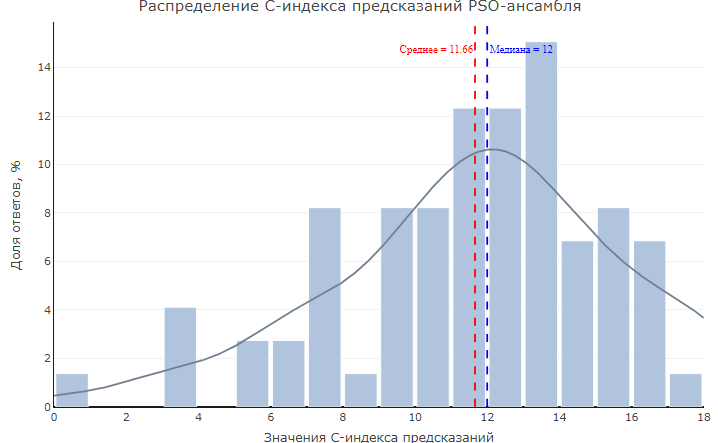
\includegraphics[width=0.95\linewidth]{figures/Cindex_distr_PSO_regr.png}
    \caption{Распределение значений C-индекса для предсказаний PSO-ансамбля регрессоров}
    \label{fig:cindex_distr}
\end{figure}

Сравнение моделей базовых классификаторов в разрезе трех главных подходов для классификации показано в таблице~\ref{tab:classif_res}. Сравнение производилось по метрике Top-K точность. Подходы \emph{multiclass} и \emph{multilabel} показывают схожие результаты и опережают подход \emph{label powerset} по метрикам точности Top-1 и Top-2. Можно заметить, что большинство моделей в 98--100\% случаев верно предсказывают в тройке кодов хотя бы один код, который действительно есть в фактических данных в \emph{верхней триаде}; в 70\% и более угадываются хотя бы два кода. Лишь примерно в 15\% правильно предсказываются все три кода одновременно. 

\renewcommand{\g}[1]{\gradientcelld{#1}{8}{10.8}{11.7}{low}{mid}{high}{70}}

\begingroup
    \fontsize{8pt}{9pt}\selectfont
    \setlength{\tabcolsep}{0pt}
    \begin{table}
      \centering
      \caption{Сравнение методов подбора весов ансамбля классификаторов}
      \label{tab:clsf_ensemble}
      \begin{tabular*}{\textwidth}{@{\extracolsep{\fill}}
        >{\raggedright\arraybackslash}m{8cm} 
        *{3}{>{\centering\arraybackslash}m{2.75cm}} @{}}
        \toprule
        \textbf{Метод подбора весов}
          & \textbf{Multiclass}
          & \textbf{Multilabel}
          & \textbf{Label Powerset} \\
        \midrule
        Равные веса всех моделей      & \g{10.663} & \g{10.888} & \g{10.563} \\
        Вектор Шэпли (Shap)           & \g{10.563} & \g{11.038} & \g{10.525} \\
        Частичный перебор по сетке    & \g{11.213} & \g{11.488} & \g{11.525} \\
        Квадратичная оптимизация (QP) & \g{10.488} & \g{10.638} & \g{10.650} \\
        Генетический алгоритм (GA)    & \g{11.263} & \g{11.313} & \g{11.213} \\
        Метод роя частиц (PSO)        & \g{11.263} & \g{11.625} & \g{11.525} \\
        Координатный спуск            & \g{11.200} & \g{11.275} & \g{10.425} \\
        \bottomrule
      \end{tabular*}
    \end{table}
\endgroup


В таблице~\ref{tab:best_classif} приведено сравнение лучших базовых моделей классификации. На первом месте с $\text{C‑index}~=~10.838$ метод k-ближайших соседей (подход \emph{multilabel}), за ним логистическая Lasso-регрессия (\emph{multiclass}) с $\text{C‑index}~=~10.663$.

\begin{table}
    \setlength{\tabcolsep}{0pt}
    \centering
    \caption{Весовые коэффициенты моделей и C‑индекс для PSO}
    \label{tab:clsf_pso_w}
    \begin{tabular*}{\textwidth}{@{\extracolsep{\fill}} 
          >{\centering\arraybackslash}p{1.5cm}
          *{5}{c}>{\centering\arraybackslash}p{1.3cm}
          >{\raggedright\arraybackslash}p{1.2cm}
        @{}}
          \toprule
          \textbf{Подбор} & \multicolumn{5}{c}{\textbf{Веса моделей}} & \textbf{\quad C-}\\
          \cmidrule(lr){2-6}
          \textbf{весов} & kNN & SVM & Logit L1 & XGBoost & LightGBM & \textbf{индекс}\\
          \midrule
          PSO & 0.291 & 0.164 & 0.191 & 0.183 & 0.151 & 11.625 \\
          \bottomrule
    \end{tabular*}
\end{table}


Сравнение методов подбора весов ансамбля классификаторов представлено в таблице~\ref{tab:clsf_ensemble}. Лучшим методом подбора весов для моделей линейного блендинга (взвешенного ансамблирования) является метод роя частиц (PSO), $\text{C‑index}~=~11.625$. В таблице~\ref{tab:clsf_pso_w} приведены веса классификаторов, которые определены с помощью PSO: наибольший вклад вносят kNN и L1-регрессия. Таким образом, результаты лучшего взвешенного ансамбля классификаторов лишь немного хуже лучшего регрессионного ансамбля.

\renewcommand{\g}[1]{\gradientcelld{#1}{7}{9.6}{11.5}{low}{mid}{high}{70}}
\newcommand{\gndcg}[1]{\gradientcelld{#1}{0.25}{0.54}{0.7}{low}{mid}{high}{70}}

\begingroup
    \setlength{\tabcolsep}{0pt}
    \begin{table}
        \fontsize{14pt}{14pt}\selectfont
        \centering
        \caption{Сравнение моделей ранжирования}
        \label{tab:rank}
        \begin{tabular*}{\textwidth}{@{\extracolsep{\fill}} 
          >{\raggedright\arraybackslash}p{3cm}  % Функция потерь
          | *{3}{>{\centering\arraybackslash}p{2.2cm}}  % C‑индекс
          | *{3}{>{\centering\arraybackslash}p{2.2cm}}  % NDCG@3
        }
          \toprule
            \multicolumn{1}{c|}{\textbf{Функция}}  
              & \multicolumn{3}{c|}{\textbf{C‑индекс}} 
              & \multicolumn{3}{c}{\textbf{NDCG@3}} \\
            \cmidrule(lr){2-4} \cmidrule(lr){5-7}
            \multicolumn{1}{c|}{\textbf{потерь}}  
            & Deep \& Cross 
            & Trans\-former 
            & MLP 
            & Deep \& Cross 
            & Trans\-former 
            & MLP \\
          \midrule
          ApproxNDCG   & \g{10.025} & \g{8.888}  & \g{9.150}  & \gndcg{0.539} & \gndcg{0.439} & \gndcg{0.388} \\
          LambdaRank   & \g{9.963}  & \g{9.675}  & \g{9.650}  & \gndcg{0.527} & \gndcg{0.489} & \gndcg{0.543} \\
          ListNet@1    & \g{9.650}  & \g{10.325} & \g{10.438} & \gndcg{0.504} & \gndcg{0.628} & \gndcg{0.653} \\
          ListNet@3    & \g{9.450}  & \g{9.950}  & \g{10.788} & \gndcg{0.458} & \gndcg{0.622} & \gndcg{0.638} \\
          \bottomrule
        \end{tabular*}
    \end{table}
\endgroup


Сравнение моделей ранжирования отражено в таблице~\ref{tab:rank}. Лучшая из моделей, многослойный перцептрон с функцией потерь ListNet@3, показывает $\text{C‑index}~=~10.788$, что заведомо хуже, чем лучшие из базовых регрессоров и классификаторов.

\renewcommand{\g}[1]{\gradientcelld{#1}{10}{10.65}{11.7}{low}{mid}{high}{60}}

\begin{table}[!b]
    \fontsize{14pt}{18pt}\selectfont
    \setlength{\tabcolsep}{0pt}
    \centering
    \caption{Обзор лучших моделей для каждого типа задач}
    \label{tab:summary}
    \begin{tabular*}{\textwidth}{@{\extracolsep{\fill}}
        >{\raggedright\arraybackslash}m{4.0cm}   % Тип задач
        | >{\raggedright\arraybackslash}m{3.7cm} % Подход
        | >{\raggedright\arraybackslash}m{5.9cm}   % Лучшая модель
        | >{\centering\arraybackslash}m{2.65cm}     % C‑индекс
        @{}}
        \toprule
        \multicolumn{1}{c|}{\textbf{Тип задач}}
          & \multicolumn{1}{c|}{\textbf{Подход}}
          & \multicolumn{1}{c|}{\textbf{Лучшая модель}}
          & \multicolumn{1}{c}{\textbf{C-индекс}} \\
        \specialrule{0.2pt}{1pt}{1pt}
        Регрессия       & Блендинг, mo
                        & PSO (L1-регрессия, пошаговая регрессия, CatBoost, ExtraTrees)
                        & \g{11.663} \\
        \specialrule{0.2pt}{1pt}{1pt}
        Классификация   & Блендинг, ml
                        & PSO (kNN, SVM, логистич. L1-регр., XGBoost, LightGBM и др.)
                        & \g{11.625} \\
        \specialrule{0.2pt}{1pt}{1pt}
        Регрессия       & Блендинг, chain
                        & PSO
                        & \g{11.613} \\
        \specialrule{0.2pt}{1pt}{1pt}
        Классификация   & Блендинг, lp
                        & PSO / поиск по сетке
                        & \g{11.525} \\
        \specialrule{0.2pt}{1pt}{1pt}
        Классификация   & Блендинг, mc
                        & Генетический алг. / PSO
                        & \g{11.263} \\
        \specialrule{0.2pt}{1pt}{1pt}
        Регрессия       & Multioutput
                        & L1-регрессия
                        & \g{11.175} \\
        \specialrule{0.2pt}{1pt}{1pt}
        Регрессия       & Chain
                        & L2-регрессия
                        & \g{11.062} \\
        \specialrule{0.2pt}{1pt}{1pt}
        Классификация   & Multilabel
                        & kNN
                        & \g{10.838} \\
        \specialrule{0.2pt}{1pt}{1pt}
        Ранжирование    & Списочное
                        & MLP с ListNet@3
                        & \g{10.788} \\
        \specialrule{0.2pt}{1pt}{1pt}
        Классификация   & Multiclass
                        & Логистич. L1-регрессия
                        & \g{10.663} \\
        \bottomrule
    \end{tabular*}
    \begin{minipage}{\textwidth}
      \small
      \textit{Обозначения:\\
      \hspace*{1em}mo~--- Multioutput, ml~--- Multilabel, lp~--- Label Powerset, mc~--- Multiclass,\\
      \hspace*{1em}MLP~--- многослойный перцептрон, PSO~--- метод роя частиц,\\
      \hspace*{1em}SVM~--- метод опорных векторов, kNN~--- метод k-ближайших соседей}
    \end{minipage}
\end{table}

Лучшие из моделей по каждому рассматриваемому типу задач приведены в таблице~\ref{tab:summary}. Двумя лучшими моделями оказались линейные блендинги, веса которых подобраны методом роя частиц: это подходы \emph{multioutput} для регрессии ($\text{C‑index}~=~11.663$) и \emph{multilabel} для классификации ($\text{C‑index}~=~11.625$). Результаты базовых моделей уступают результатам их комбинаций в виде взвешенных ансамблей. 

\subsection{Сравнение подходов к восстановлению данных тестов}

\renewcommand{\g}[1]{\gradientcelld{#1}{7}{9.6}{10.9}{low}{mid}{high}{70}}
  
  \begingroup
    \fontsize{8pt}{9pt}\selectfont
    \setlength{\tabcolsep}{3pt}
    \begin{table}[!b]
      \centering
      \caption{Восстановление значений незаполненных психометрических тестов}
      \label{tab:impute}
      \begin{tabular*}{\textwidth}{@{\extracolsep{\fill}} 
        >{\raggedright\arraybackslash}m{6cm} 
        *{4}{>{\centering\arraybackslash}m{2.4cm}}
      @{}}
        \toprule
        \textbf{Модель-регрессор}
          & \textbf{MICE}
          & \textbf{Soft Impute}
          & \textbf{Маски}
          & \textbf{Ансам\-бли} \\
        \midrule
        Регрессия Lasso (L1)   & \g{9.191} & \g{10.248}  & \g{9.998} & \g{9.866} \\
        Пошаговая регрессия    & \g{9.608} & \g{10.183}  & \g{9.978} & \g{10.082}\\
        Random Forest          & \g{9.518} & \g{10.136}  & \g{9.819} & \g{9.712} \\
        LightGBM               & \g{9.372} & \g{10.086}  & \g{9.686} & \g{9.594} \\
        Линейная регр. (OLS)   & \g{9.407} & \g{10.021}  & \g{9.876} & \g{10.012}\\
        Регрессия Ridge (L2)   & \g{9.442} & \g{9.770}   & \g{9.868} & \g{9.933} \\
        ExtraTrees             & \g{9.101} & \g{9.823}   & \g{9.870} & \g{9.808} \\
        Метод опорных векторов & \g{9.221} & \g{9.814}   & \g{9.864} & \g{9.760} \\
        CatBoost               & \g{9.131} & \g{9.814}   & \g{9.835} & \g{9.461} \\
        kNN                    & \g{9.372} & \g{9.834}   & \g{9.830} & \g{9.377} \\
        XGBoost                & \g{8.769} & \g{9.571}   & \g{9.267} & \g{9.614} \\
        Constant baseline      & \g{9.000} & \g{9.000}   & \g{9.000} & \g{9.000} \\
        \bottomrule
      \end{tabular*}
    \end{table}
  \endgroup

Результаты предсказания регрессионных моделей с использованием различных подходов к восстановлению значений незаполненных психометрических тестов представлены в таблице~\ref{tab:impute}. Лучшие базовые модели для восстановления результатов~--- это Lasso- и пошаговый регрессоры в сочетании с подходом мягкого матричного восстановления данных ($\text{C‑index}~=~10.248$ и $\text{C‑index}~=~10.183$). Ансамблирование моделей, обученных на данных заполненных тестов по отдельности, затем объединенных воедино в зависимости от наличия того или иного теста, показывает следующие результаты: наибольшее значение С-индекса для пошаговой моделей регрессии лишь немного хуже подхода \emph{Soft Impute}: $\text{C‑index}~=~10.082$, однако ансамблевый подход по отдельным тестам требует обучения для всех 31 комбинации наличия тестов. Применение масочного подхода к восстановлению данных в меньшей степени зависит от выбора базовой модели. Хуже всего себя показывает подход множественной импутации (\emph{MICE}).
\renewcommand{\g}[1]{\gradientcelld{#1}{9}{10.25}{11}{low}{mid}{high}{70}}

\begin{table}
  \setlength{\tabcolsep}{0pt}
  \centering
  \caption{Весовые коэффициенты моделей и C-индекс при разных методах подбора весов для ансамблей на восстановленных данных}
  \label{tab:impute_ens}
  \begin{tabular*}{\textwidth}{@{\extracolsep{\fill}} 
        >{\raggedright\arraybackslash}m{1.5cm}
        *{5}{c}
        >{\centering\arraybackslash}m{1.9cm}
      @{}}
    \toprule
    \textbf{Подбор} 
      & \multicolumn{5}{c}{\textbf{Веса моделей}} 
      & \textbf{C-}\\
    \cmidrule(lr){2-6}
    \textbf{весов} 
      & \textbf{Lasso L1} 
      & \textbf{Пошаг.} 
      & \textbf{LightGBM} 
      & \textbf{Случ. лес} 
      & \textbf{kNN} 
      & \textbf{индекс} \\
    \midrule
    PSO    & 0.001 & 0.481 & 0.038 & 0.475 & 0.005 & \g{10.740} \\
    Grid   & 0.000 & 0.500 & 0.000 & 0.500 & 0.000 & \g{10.657} \\
    GA     & 0.281 & 0.369 & 0.109 & 0.189 & 0.052 & \g{10.401} \\
    Спуск  & 0.019 & 0.422 & 0.067 & 0.305 & 0.187 & \g{10.245} \\
    QP     & 0.050 & 0.000 & 0.390 & 0.007 & 0.553 & \g{10.065} \\
    Равные & 0.200 & 0.200 & 0.200 & 0.200 & 0.200 & \g{10.053} \\
    Шэпли  & 0.247 & 0.185 & 0.206 & 0.179 & 0.183 & \g{10.047} \\
    \bottomrule
  \end{tabular*}
  \vspace{0.5em}
  \begin{minipage}{\textwidth}
    \small
    \textit{Обозначения:\\
    \hspace*{1em}PSO~--- метод роя частиц, Grid~--- частичный перебор по сетке,\\
    \hspace*{1em}GA~--- генетический алгоритм, спуск~--- координатный спуск,\\
    \hspace*{1em}QP~--- квадратичная оптимизация, пошаг. ~--- пошаговая регрессия,\\
    \hspace*{1em}случ. лес~--- случайный лес (Random Forest), kNN~--- метод k-ближайших соседей}
  \end{minipage}
\end{table}



В таблице~\ref{tab:impute_ens} был применен лучший из подходов к восстановлению данных, мягкое матричное восстановление, и проведен вычислительный эксперимент с регрессионными моделями, как если бы данные были полными. Для ансамблирования были взяты топ-5 моделей, показавших наибольшие значения меры сходства на этих данных по отдельности. Наилучший результат достигнут при подборе весов для ансамбля с помощью метода роя частиц (\emph{PSO}): $\text{C‑index}~=~10.74$, где наибольший вклад вносят модели пошаговой регрессии (48.1\%) и случайного леса (47.5\%). Таким образом, ансамблирование позволяет значительно улучшить результаты предсказания на восстановленных данных, однако значения меры сходства на восстановленных данных ниже, чем на полных данных для аналогичных моделей регрессии и классификации.
% !TeX spellcheck = ru_RU
% !TEX root = vkr.tex

\section*{Заключение}

В ходе работы была достигнута поставленная цель: разработан инструмент для автоматизации профориентации на основе предсказания кода Голланда по неполным результатам психометрических тестов личности. Для выполнения цели были решены следующие задачи:
% [noitemsep, topsep=0pt, parsep=0pt, partopsep=0pt]
\begin{enumerate}
    \item Разработаны и реализованы математические модели модуля восстановления пропусков результатов психометрических тестов: \emph{MICE}, маски, ансамбли по набору заполненных тестов и метод мягкой импутации, который в сочетании с PSO-ансамблем регрессоров показал наибольший C-индекс:~$10.74$.

    \item Реализованы подходы к определению кода Голланда: многоцелевая регрессия (\emph{multioutput}, \emph{chain}), классификация (\emph{multiclass}, \emph{multilabel}, \emph{label powerset}), списочное ранжирование.

    \item Разработан модуль формирования взвешенного ансамбля моделей на основе методов подбора весов: метод роя частиц (PSO), равные веса, частичный перебор по сетке, вектор Шэпли, квадратичная оптимизация, генетический алгоритм и координатный спуск.
    
    \item Проведен сравнительный анализ моделей предсказания кодов Голланда; лучшие результаты у моделей линейного блендинга с оптимизацией весов моделей методом роя частиц:
      \begin{itemize}[noitemsep, topsep=0pt, parsep=0pt, partopsep=0pt]
        \item ансамбль \emph{multioutput}‑регрессоров: Lasso- и пошаговая регрессии, CatBoost, ExtraTrees ($\text{C‑index}~=~11.663$);
        \item ансамбль \emph{multilabel}‑классификаторов: kNN, SVM, логистическая Lasso-регрессия, XGBoost, LightGBM и др. ($\text{C‑index}~=~11.625$);
        \item лучшая базовая модель~--- L1-регрессия со множественными выходами ($\text{C‑index}~=~11.175$);
        \item показано превосходство классических методов машинного обучения над нейросетевыми в данной задаче.
      \end{itemize}

    \item Создан прототип инструмента для определения профориентационных предпочтений на основе R Shiny.
\end{enumerate}

Исходный код всего проекта представлен в GitHub-репозитории\footnote{\quad GitHub: Предсказание кода Голланда (RIASEC) по результатам психометрических тестов личности. URL: \url{https://github.com/ExP98/Diploma_Holland} (дата обращения: 17.05.2025).}. Отдельные аспекты вычислительного эксперимента, связанные с решением задач регрессии и классификации, ранее были представлены на XXVIII Международной конференции по мягким вычислениям и измерениям SCM'2025.


\setmonofont{CMU Typewriter Text}
%% в .cls заменить в bibliographystyle plain на tex/ugost2008l.bst при конечной компиляции
\bibliography{vkr.bib}

\clearpage

\begin{appendices}
    \appendix
    \renewcommand{\thesection}{\Alph{section}}

    % Перенастраиваем заголовки \section так, чтобы для приложений было "Приложение A. Название"
    \titleformat{\section}[block]
      {\normalfont\Large\bfseries}{\appendixname\ \thesection.}{1em}{}

    \begin{landscape}
        \section{Описание психометрических тестов}
        \label{app:psytests}
        \small
        % psytests_desc_stats.tex
% Описание: таблица описательной статистики психометрических тестов
% Содержит только тело таблицы longtable

% Для объединения ячеек в первом столбце требуется пакет multirow
\begin{longtable}{
>{\raggedright\arraybackslash}p{3.2cm} 
>{\raggedright\arraybackslash}p{8.8cm} 
>{\ttfamily\raggedright\arraybackslash}p{1cm} 
r
>{\raggedleft\arraybackslash}p{2.8cm} 
>{\raggedleft\arraybackslash}p{3.1cm} 
r r}
\caption{Психометрические тесты: описательная статистика}
\label{tab:psytests_desc_stats} \\
\toprule
\textbf{Опросник} & \textbf{Признак} & \textbf{Код} & \textbf{N} & \textbf{Mean (SD)} & \textbf{Median (IQR)} & \textbf{Min} & \textbf{Max} \\
\midrule
\endfirsthead

\caption[]{Психометрические тесты: описательная статистика (продолжение)} \\
\toprule
\textbf{Опросник} & \textbf{Признак} & \textbf{Код} & \textbf{N} & \textbf{Mean (SD)} & \textbf{Median (IQR)} & \textbf{Min} & \textbf{Max} \\
\midrule
\endhead

\midrule
\multicolumn{8}{r}{Продолжение на следующей странице} \\
\midrule
\endfoot

\bottomrule
\endlastfoot

% Данные по 16 факторному опроснику Кеттелла
\multirow[t]{16}{=}{16-факторный опросник Кеттелла} & Открытость -- Замкнутость & CT\_1 & 993 & 9,91 (3,67) & 10 (7--12) & 0 & 19 \\
 & Эмоцион. стабильность -- Неустойчивость & CT\_2 & 993 & 12,99 (4,73) & 13 (10--16) & 0 & 26 \\
 & Независимость -- Податливость & CT\_3 & 993 & 12,84 (4,06) & 13 (10--16) & 1 & 25 \\
 & Беспечность -- Озабоченность & CT\_4 & 993 & 12,25 (4,35) & 12 (9--15) & 2 & 25 \\
 & Сознательность -- Беспринципность & CT\_5 & 993 & 10,61 (3,56) & 11 (8--13) & 1 & 20 \\
 & Смелость -- Застенчивость & CT\_6 & 993 & 10,88 (5,93) & 11 (6--15) & 0 & 26 \\
 & Чувственность -- Твердость & CT\_7 & 993 & 11,99 (3,71) & 12 (10--15) & 1 & 20 \\
 & Подозрительность -- Доверчивость & CT\_8 & 993 & 10,72 (3,55) & 11 (8--13) & 0 & 20 \\
 & Мечтательность -- Практичность & CT\_9 & 993 & 10,84 (3,02) & 11 (9--13) & 2 & 20 \\
 & Утонченность -- Простота & CT\_10 & 993 & 10,06 (2,99) & 10 (8--12) & 2 & 20 \\
 & Склонность к чувству вины -- Спокойная самоуверенность & CT\_11 & 993 & 13,99 (4,99) & 14 (10--18) & 0 & 26 \\
 & Радикализм -- Консерватизм & CT\_12 & 993 & 10,32 (2,97) & 10 (8--12) & 0 & 20 \\
 & Самостоятельность -- Зависимость от группы & CT\_13 & 993 & 12,60 (3,51) & 13 (10--15) & 1 & 20 \\
 & Сильная воля -- Недостаток самоконтроля & CT\_14 & 993 & 11,42 (3,43) & 12 (9--14) & 1 & 20 \\
 & Внутренняя напряженность -- Расслабленность & CT\_15 & 993 & 14,46 (5,25) & 15 (11--18) & 0 & 26 \\
 & Развитое мышление -- Ограниченное мышление & CT\_16 & 993 & 7,69 (2,32) & 8 (6--9) & 1 & 13 \\
\cline{1-8}
% Данные по личностному опроснику Айзенка
\multirow[t]{4}{=}{Личностный опросник Айзенка} & Экстраверсия & EY\_1 & 1200 & 11,2 (5,38) & 11 (7--15) & 0 & 24 \\
 & Психотизм & EY\_2 & 1200 & 6,29 (3,31) & 6 (4--8) & 0 & 22 \\
 & Нейротизм & EY\_3 & 1200 & 16,25 (5,74) & 17 (12--21) & 1 & 25 \\
 & Искренность & EY\_4 & 1200 & 10,79 (4,36) & 11 (8--14) & 0 & 25 \\
\cline{1-8}
% Данные по опроснику Леонгарда-Шмишека
\multirow[t]{10}{=}{Опросник Леонгарда-Шмишека} & Гипертимность & LN\_1 & 998 & 12,84 (6,47) & 12 (9--18) & 0 & 24 \\
 & Дистимность & LN\_2 & 998 & 14,95 (4,07) & 16 (12--18) & 2 & 24 \\
 & Циклотимность & LN\_3 & 998 & 14,71 (5,19) & 15 (12--18) & 0 & 24 \\
 & Неуравновешенность & LN\_4 & 998 & 12,27 (4,83) & 12 (8--16) & 0 & 24 \\
 & Застревание & LN\_5 & 998 & 11,77 (6,03) & 12 (6--15) & 0 & 24 \\
 & Эмотивность & LN\_6 & 998 & 14,93 (5,85) & 15 (9--18) & 0 & 24 \\
 & Экзальтированность & LN\_7 & 998 & 13,92 (4,6) & 14 (10--18) & 2 & 24 \\
 & Тревожность & LN\_8 & 998 & 13,54 (5,53) & 15 (9--18) & 0 & 24 \\
 & Педантичность & LN\_9 & 998 & 13,10 (4,72) & 12 (9--15) & 0 & 24 \\
 & Демонстративность & LN\_10 & 998 & 15,26 (5,96) & 18 (12--18) & 0 & 24 \\
\cline{1-8}
% Данные по пятифакторному опроснику личности
\multirow[t]{5}{=}{Пятифакторный опросник личности} & Экстраверсия -- интроверсия & BF\_1 & 891 & 43,54 (11,51) & 43 (35--51) & 16 & 75 \\
 & Привязанность -- обособленность & BF\_2 & 891 & 49,76 (11,78) & 50 (42--58) & 15 & 75 \\
 & Самоконтроль -- импульсивность & BF\_3 & 891 & 51,38 (11,34) & 51 (43--60) & 15 & 75 \\
 & Эмоциональная устойчивость -- эмоциональная неустойчивость & BF\_4 & 891 & 52,58 (13,96) & 54 (44--63,5) & 15 & 75 \\
 & Экспрессивность -- практичность & BF\_5 & 891 & 54,63 (8,68) & 55 (49--61) & 15 & 75 \\
\cline{1-8}
% Данные по ценностному опроснику Шварца
\multirow[t]{20}{=}{Ценностный опросник Шварца} & Универсализм -- НИ & SC\_1 & 747 & 38,66 (10) & 40 (33--46) & -8 & 56 \\
 & Безопасность -- НИ & SC\_2 & 747 & 25,12 (6,24) & 26 (22--29) & -5 & 35 \\
 & Власть -- НИ & SC\_3 & 747 & 15,69 (6,58) & 16 (11--20) & -2 & 28 \\
 & Гедонизм -- НИ & SC\_4 & 747 & 14,61 (4,8) & 15 (12--18) & -2 & 21 \\
 & Самостоятельность -- НИ & SC\_5 & 747 & 26,65 (5,35) & 27 (24--30) & 0 & 35 \\
 & Стимуляция -- НИ & SC\_6 & 747 & 11,36 (5,23) & 12 (8--15) & -3 & 21 \\
 & Конформность -- НИ & SC\_7 & 747 & 17,04 (5,98) & 18 (14--21) & -4 & 28 \\
 & Традиция -- НИ & SC\_8 & 747 & 17,36 (8,16) & 18 (12--23) & -5 & 35 \\
 & Доброта -- НИ & SC\_9 & 747 & 24,06 (6,98) & 25 (20--29) & -3 & 35 \\
 & Достижение -- НИ & SC\_10 & 747 & 19,49 (5,53) & 20 (16--24) & -3 & 28 \\
 & Самостоятельность -- ИП & SC\_11 & 747 & 11,15 (3,44) & 12 (9--14) & -1 & 16 \\
 & Власть -- ИП & SC\_12 & 747 & 4,63 (3,8) & 4 (2--8) & -3 & 12 \\
 & Универсализм -- ИП & SC\_13 & 747 & 13,87 (5,8) & 14 (10--19) & -6 & 24 \\
 & Достижение -- ИП & SC\_14 & 747 & 8,61 (4,54) & 9 (5--12) & -4 & 16 \\
 & Безопасность -- ИП & SC\_15 & 747 & 10,69 (5,03) & 11 (7--14) & -5 & 20 \\
 & Стимуляция -- ИП & SC\_16 & 747 & 5,31 (3,49) & 5 (3--8) & -3 & 12 \\
 & Конформность -- ИП & SC\_17 & 747 & 6,43 (4,46) & 7 (3--10) & -4 & 16 \\
 & Традиция -- ИП & SC\_18 & 747 & 4,46 (4,44) & 4 (1--7) & -4 & 16 \\
 & Гедонизм -- ИП & SC\_19 & 747 & 7,38 (3,35) & 8 (5--10) & -3 & 12 \\
 & Доброта -- ИП & SC\_20 & 747 & 8,27 (4,37) & 9 (5--11) & -4 & 16 \\
\cline{1-8}
% Данные по тесту Голланда
\multirow[t]{6}{=}{Тест Голланда} & Реалистический (R) & HL\_1 & 1278 & 6,42 (2,33) & 6 (5--8) & 0 & 14 \\
 & Исследовательский (I) & HL\_2 & 1278 & 7,19 (2,18) & 7 (6--9) & 2 & 13 \\
 & Артистический (A) & HL\_3 & 1278 & 7,09 (2,07) & 7 (6--9) & 1 & 13 \\
 & Социальный (S) & HL\_4 & 1278 & 6,67 (2,04) & 7 (5--8) & 1 & 13 \\
 & Предприимчивый (E) & HL\_5 & 1278 & 7,04 (2,34) & 7 (5--9) & 1 & 13 \\
 & Традиционный (C) & HL\_6 & 1278 & 7,59 (2,78) & 8 (6--10) & 0 & 14 \\
\end{longtable}

    \end{landscape}

    \begin{landscape}
        \section{Интерфейс прототипа приложения}
        \label{app:ui}
        \begin{figure}[!h]
            \centering
            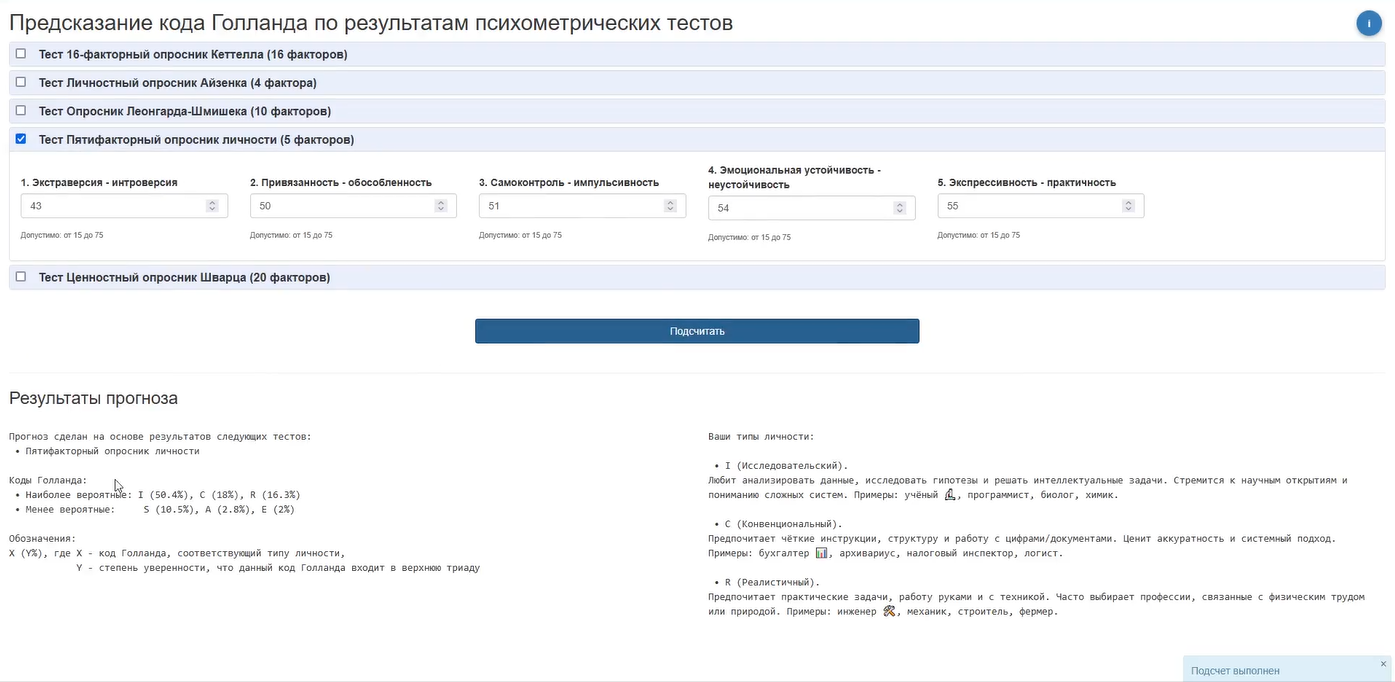
\includegraphics[width=1.0\linewidth]{figures/UI2.png}
            \caption{Интерфейс прототипа инструмента профориентации}
            \label{fig:ui2}
        \end{figure}
    \end{landscape}

\end{appendices}

\end{document}
